\documentclass[twoside]{book}

% Packages required by doxygen
\usepackage{fixltx2e}
\usepackage{calc}
\usepackage{doxygen}
\usepackage[export]{adjustbox} % also loads graphicx
\usepackage{graphicx}
\usepackage[utf8]{inputenc}
\usepackage{makeidx}
\usepackage{multicol}
\usepackage{multirow}
\PassOptionsToPackage{warn}{textcomp}
\usepackage{textcomp}
\usepackage[nointegrals]{wasysym}
\usepackage[table]{xcolor}

% Font selection
\usepackage[T1]{fontenc}
\usepackage[scaled=.90]{helvet}
\usepackage{courier}
\usepackage{amssymb}
\usepackage{sectsty}
\renewcommand{\familydefault}{\sfdefault}
\allsectionsfont{%
  \fontseries{bc}\selectfont%
  \color{darkgray}%
}
\renewcommand{\DoxyLabelFont}{%
  \fontseries{bc}\selectfont%
  \color{darkgray}%
}
\newcommand{\+}{\discretionary{\mbox{\scriptsize$\hookleftarrow$}}{}{}}

% Page & text layout
\usepackage{geometry}
\geometry{%
  a4paper,%
  top=2.5cm,%
  bottom=2.5cm,%
  left=2.5cm,%
  right=2.5cm%
}
\tolerance=750
\hfuzz=15pt
\hbadness=750
\setlength{\emergencystretch}{15pt}
\setlength{\parindent}{0cm}
\setlength{\parskip}{3ex plus 2ex minus 2ex}
\makeatletter
\renewcommand{\paragraph}{%
  \@startsection{paragraph}{4}{0ex}{-1.0ex}{1.0ex}{%
    \normalfont\normalsize\bfseries\SS@parafont%
  }%
}
\renewcommand{\subparagraph}{%
  \@startsection{subparagraph}{5}{0ex}{-1.0ex}{1.0ex}{%
    \normalfont\normalsize\bfseries\SS@subparafont%
  }%
}
\makeatother

% Headers & footers
\usepackage{fancyhdr}
\pagestyle{fancyplain}
\fancyhead[LE]{\fancyplain{}{\bfseries\thepage}}
\fancyhead[CE]{\fancyplain{}{}}
\fancyhead[RE]{\fancyplain{}{\bfseries\leftmark}}
\fancyhead[LO]{\fancyplain{}{\bfseries\rightmark}}
\fancyhead[CO]{\fancyplain{}{}}
\fancyhead[RO]{\fancyplain{}{\bfseries\thepage}}
\fancyfoot[LE]{\fancyplain{}{}}
\fancyfoot[CE]{\fancyplain{}{}}
\fancyfoot[RE]{\fancyplain{}{\bfseries\scriptsize Generated by Doxygen }}
\fancyfoot[LO]{\fancyplain{}{\bfseries\scriptsize Generated by Doxygen }}
\fancyfoot[CO]{\fancyplain{}{}}
\fancyfoot[RO]{\fancyplain{}{}}
\renewcommand{\footrulewidth}{0.4pt}
\renewcommand{\chaptermark}[1]{%
  \markboth{#1}{}%
}
\renewcommand{\sectionmark}[1]{%
  \markright{\thesection\ #1}%
}

% Indices & bibliography
\usepackage{natbib}
\usepackage[titles]{tocloft}
\setcounter{tocdepth}{3}
\setcounter{secnumdepth}{5}
\makeindex

% Hyperlinks (required, but should be loaded last)
\usepackage{ifpdf}
\ifpdf
  \usepackage[pdftex,pagebackref=true]{hyperref}
\else
  \usepackage[ps2pdf,pagebackref=true]{hyperref}
\fi
\hypersetup{%
  colorlinks=true,%
  linkcolor=blue,%
  citecolor=blue,%
  unicode%
}

% Custom commands
\newcommand{\clearemptydoublepage}{%
  \newpage{\pagestyle{empty}\cleardoublepage}%
}

\usepackage{caption}
\captionsetup{labelsep=space,justification=centering,font={bf},singlelinecheck=off,skip=4pt,position=top}

%===== C O N T E N T S =====

\begin{document}

% Titlepage & ToC
\hypersetup{pageanchor=false,
             bookmarksnumbered=true,
             pdfencoding=unicode
            }
\pagenumbering{roman}
\begin{titlepage}
\vspace*{7cm}
\begin{center}%
{\Large Terminal-\/based Motion-\/controlled Game Engine using Open\+CV }\\
\vspace*{1cm}
{\large Generated by Doxygen 1.8.11}\\
\end{center}
\end{titlepage}
\clearemptydoublepage
\tableofcontents
\clearemptydoublepage
\pagenumbering{arabic}
\hypersetup{pageanchor=true}

%--- Begin generated contents ---
\chapter{Terminal-\/based Motion-\/controlled Game Engine using Open\+CV}
\label{md_README}
\hypertarget{md_README}{}
\subsection*{Update the Open\+CV Submodule}


\begin{DoxyEnumerate}
\item {\ttfamily cd opencv}
\item {\ttfamily git submodule update -\/-\/init}
\end{DoxyEnumerate}

\subsection*{Instructions to Build Open\+CV and Link to Project}


\begin{DoxyEnumerate}
\item {\ttfamily cd opencv}
\item {\ttfamily mkdir build}
\item {\ttfamily cd build}
\item {\ttfamily cmake -\/D C\+M\+A\+K\+E\+\_\+\+B\+U\+I\+L\+D\+\_\+\+T\+Y\+PE=Release ..}
\item {\ttfamily make -\/j\mbox{[}n\mbox{]}} where {\ttfamily \mbox{[}n\mbox{]}} is the number of threads to use.
\item {\ttfamily cd ../..}
\item {\ttfamily cmake .}
\item {\ttfamily cmake-\/gui}
\item Set the {\ttfamily Open\+C\+V\+\_\+\+D\+IR} parameter to point to the {\ttfamily opencv} folder.
\item Click {\ttfamily Configure} and {\ttfamily Generate} and then close.
\item {\ttfamily make} 
\end{DoxyEnumerate}
\chapter{Data Structure Index}
\section{Data Structures}
Here are the data structures with brief descriptions\+:\begin{DoxyCompactList}
\item\contentsline{section}{\hyperlink{structascii__t}{ascii\+\_\+t} \\*A struct to hold information about an A\+S\+C\+II sprite }{\pageref{structascii__t}}{}
\item\contentsline{section}{\hyperlink{structcalibration__t}{calibration\+\_\+t} \\*A struct to hold the H\+SV values of the calibrated skin colour }{\pageref{structcalibration__t}}{}
\item\contentsline{section}{\hyperlink{structhands__t}{hands\+\_\+t} \\*A struct that holds information about the positions of hands }{\pageref{structhands__t}}{}
\item\contentsline{section}{\hyperlink{structobject__list__elem}{object\+\_\+list\+\_\+elem} \\*A struct to store the state of an object }{\pageref{structobject__list__elem}}{}
\item\contentsline{section}{\hyperlink{structobject__list__elem__t}{object\+\_\+list\+\_\+elem\+\_\+t} }{\pageref{structobject__list__elem__t}}{}
\item\contentsline{section}{\hyperlink{structobject__list__t}{object\+\_\+list\+\_\+t} \\*A struct to store a list of objects }{\pageref{structobject__list__t}}{}
\item\contentsline{section}{\hyperlink{structuchar__array__t}{uchar\+\_\+array\+\_\+t} \\*A struct to hold a unsigned char array. Also holds the size, and the standard deviation }{\pageref{structuchar__array__t}}{}
\item\contentsline{section}{\hyperlink{structvector__t}{vector\+\_\+t} \\*A vector pair struct }{\pageref{structvector__t}}{}
\end{DoxyCompactList}

\chapter{File Index}
\section{File List}
Here is a list of all documented files with brief descriptions\+:\begin{DoxyCompactList}
\item\contentsline{section}{\hyperlink{calibration_8c}{calibration.\+c} \\*Functions to calibrate colours }{\pageref{calibration_8c}}{}
\item\contentsline{section}{\hyperlink{detection_8c}{detection.\+c} \\*Functions to detect position of hands }{\pageref{detection_8c}}{}
\item\contentsline{section}{\hyperlink{main_8cpp}{main.\+cpp} \\*Main file for motion-\/controlled games }{\pageref{main_8cpp}}{}
\item\contentsline{section}{\hyperlink{threshold_8c}{threshold.\+c} \\*Functions to determine skin-\/coloured pixel within a frame }{\pageref{threshold_8c}}{}
\item\contentsline{section}{\hyperlink{uchar__array_8c}{uchar\+\_\+array.\+c} \\*Definition of and functions for unsigned character array }{\pageref{uchar__array_8c}}{}
\item\contentsline{section}{flappy-\/bird/\hyperlink{ascii__art_8h}{ascii\+\_\+art.\+h} \\*Header to define the \hyperlink{structascii__t}{ascii\+\_\+t} struct }{\pageref{ascii__art_8h}}{}
\item\contentsline{section}{flappy-\/bird/\hyperlink{flappy__bird_8h}{flappy\+\_\+bird.\+h} \\*Header file for flappy bird }{\pageref{flappy__bird_8h}}{}
\item\contentsline{section}{flappy-\/bird/\hyperlink{main_8c}{main.\+c} \\*Main file for flappy bird game }{\pageref{main_8c}}{}
\item\contentsline{section}{flappy-\/bird/\hyperlink{main__snake_8c}{main\+\_\+snake.\+c} \\*Main file for snake game }{\pageref{main__snake_8c}}{}
\item\contentsline{section}{flappy-\/bird/\hyperlink{object__list_8c}{object\+\_\+list.\+c} \\*Functions for using object list }{\pageref{object__list_8c}}{}
\item\contentsline{section}{flappy-\/bird/\hyperlink{object__list_8h}{object\+\_\+list.\+h} \\*Data type for storing the state of the game }{\pageref{object__list_8h}}{}
\item\contentsline{section}{flappy-\/bird/\hyperlink{snake_8c}{snake.\+c} \\*Functions for initialising and rendering a snake game }{\pageref{snake_8c}}{}
\item\contentsline{section}{flappy-\/bird/\hyperlink{snake_8h}{snake.\+h} \\*Header file for \hyperlink{snake_8c}{snake.\+c} }{\pageref{snake_8h}}{}
\end{DoxyCompactList}

\chapter{Data Structure Documentation}
\hypertarget{structascii__t}{}\section{ascii\+\_\+t Struct Reference}
\label{structascii__t}\index{ascii\+\_\+t@{ascii\+\_\+t}}


A struct to hold information about an A\+S\+C\+II sprite.  




{\ttfamily \#include $<$ascii\+\_\+art.\+h$>$}

\subsection*{Data Fields}
\begin{DoxyCompactItemize}
\item 
char $\ast$ \hyperlink{structascii__t_a78fc115bb20d9af8ba8f640200027e22}{ascii}
\item 
int \hyperlink{structascii__t_a9a0d8716acbfc50587bb8e72e97b1b39}{color}
\item 
uint16\+\_\+t \hyperlink{structascii__t_ab60ac2dac5effbff37ae096f0898ac54}{height}
\item 
uint16\+\_\+t \hyperlink{structascii__t_af246687087b404068b50c0fad93b2320}{width}
\end{DoxyCompactItemize}


\subsection{Detailed Description}
A struct to hold information about an A\+S\+C\+II sprite. 

\subsection{Field Documentation}
\index{ascii\+\_\+t@{ascii\+\_\+t}!ascii@{ascii}}
\index{ascii@{ascii}!ascii\+\_\+t@{ascii\+\_\+t}}
\subsubsection[{\texorpdfstring{ascii}{ascii}}]{\setlength{\rightskip}{0pt plus 5cm}char $\ast$ ascii\+\_\+t\+::ascii}\hypertarget{structascii__t_a78fc115bb20d9af8ba8f640200027e22}{}\label{structascii__t_a78fc115bb20d9af8ba8f640200027e22}
The A\+S\+C\+II string used to represent the object. \index{ascii\+\_\+t@{ascii\+\_\+t}!color@{color}}
\index{color@{color}!ascii\+\_\+t@{ascii\+\_\+t}}
\subsubsection[{\texorpdfstring{color}{color}}]{\setlength{\rightskip}{0pt plus 5cm}int ascii\+\_\+t\+::color}\hypertarget{structascii__t_a9a0d8716acbfc50587bb8e72e97b1b39}{}\label{structascii__t_a9a0d8716acbfc50587bb8e72e97b1b39}
The color of the A\+S\+C\+II object. This number refers to a foreground / background colour pair, which must be defined at the same time as object definition. This is done using start\+\_\+color and init\+\_\+pair. See the Linux man page for more information. \index{ascii\+\_\+t@{ascii\+\_\+t}!height@{height}}
\index{height@{height}!ascii\+\_\+t@{ascii\+\_\+t}}
\subsubsection[{\texorpdfstring{height}{height}}]{\setlength{\rightskip}{0pt plus 5cm}uint16\+\_\+t ascii\+\_\+t\+::height}\hypertarget{structascii__t_ab60ac2dac5effbff37ae096f0898ac54}{}\label{structascii__t_ab60ac2dac5effbff37ae096f0898ac54}
The height, in characters, of the A\+S\+C\+II object. \index{ascii\+\_\+t@{ascii\+\_\+t}!width@{width}}
\index{width@{width}!ascii\+\_\+t@{ascii\+\_\+t}}
\subsubsection[{\texorpdfstring{width}{width}}]{\setlength{\rightskip}{0pt plus 5cm}uint16\+\_\+t ascii\+\_\+t\+::width}\hypertarget{structascii__t_af246687087b404068b50c0fad93b2320}{}\label{structascii__t_af246687087b404068b50c0fad93b2320}
The width, in characters, of the A\+S\+C\+II object. 

The documentation for this struct was generated from the following files\+:\begin{DoxyCompactItemize}
\item 
flappy-\/bird/\hyperlink{ascii__art_8h}{ascii\+\_\+art.\+h}\item 
flappy\+\_\+bird.\+c\end{DoxyCompactItemize}

\hypertarget{structcalibration__t}{}\section{calibration\+\_\+t Struct Reference}
\label{structcalibration__t}\index{calibration\+\_\+t@{calibration\+\_\+t}}


A struct to hold the H\+SV values of the calibrated skin colour.  


\subsection*{Data Fields}
\begin{DoxyCompactItemize}
\item 
unsigned char \hyperlink{structcalibration__t_acd97fa79e525e64737d8702d397cb5f3}{h\+\_\+max}
\item 
unsigned char \hyperlink{structcalibration__t_a3e7b54f5a944fac9d22227d36df4f4b7}{h\+\_\+min}
\item 
unsigned char \hyperlink{structcalibration__t_af47b23a52b19fe1b9c097f16cf39c38e}{s\+\_\+max}
\item 
unsigned char \hyperlink{structcalibration__t_a408c4087fc2037c302179889a77c46da}{s\+\_\+min}
\item 
unsigned char \hyperlink{structcalibration__t_accaf5519bae1849954995bcdf673f1cd}{v\+\_\+max}
\item 
unsigned char \hyperlink{structcalibration__t_a05d985e74be2e4415fe9239137672741}{v\+\_\+min}
\item 
bool \hyperlink{structcalibration__t_af77af4f1701757e606eaf3e368b4e3ac}{done}
\item 
Cv\+Scalar \hyperlink{structcalibration__t_ab577a4447f9cfff14e7cb336c18fcc96}{upper}
\item 
Cv\+Scalar \hyperlink{structcalibration__t_af589528a1493701150229b3d41e13bfa}{lower}
\end{DoxyCompactItemize}


\subsection{Detailed Description}
A struct to hold the H\+SV values of the calibrated skin colour. 

\subsection{Field Documentation}
\index{calibration\+\_\+t@{calibration\+\_\+t}!done@{done}}
\index{done@{done}!calibration\+\_\+t@{calibration\+\_\+t}}
\subsubsection[{\texorpdfstring{done}{done}}]{\setlength{\rightskip}{0pt plus 5cm}bool calibration\+\_\+t\+::done}\hypertarget{structcalibration__t_af77af4f1701757e606eaf3e368b4e3ac}{}\label{structcalibration__t_af77af4f1701757e606eaf3e368b4e3ac}
True iff calibration has been done. \index{calibration\+\_\+t@{calibration\+\_\+t}!h\+\_\+max@{h\+\_\+max}}
\index{h\+\_\+max@{h\+\_\+max}!calibration\+\_\+t@{calibration\+\_\+t}}
\subsubsection[{\texorpdfstring{h\+\_\+max}{h_max}}]{\setlength{\rightskip}{0pt plus 5cm}unsigned char calibration\+\_\+t\+::h\+\_\+max}\hypertarget{structcalibration__t_acd97fa79e525e64737d8702d397cb5f3}{}\label{structcalibration__t_acd97fa79e525e64737d8702d397cb5f3}
The maximum Hue to match. \index{calibration\+\_\+t@{calibration\+\_\+t}!h\+\_\+min@{h\+\_\+min}}
\index{h\+\_\+min@{h\+\_\+min}!calibration\+\_\+t@{calibration\+\_\+t}}
\subsubsection[{\texorpdfstring{h\+\_\+min}{h_min}}]{\setlength{\rightskip}{0pt plus 5cm}unsigned char calibration\+\_\+t\+::h\+\_\+min}\hypertarget{structcalibration__t_a3e7b54f5a944fac9d22227d36df4f4b7}{}\label{structcalibration__t_a3e7b54f5a944fac9d22227d36df4f4b7}
The minimum Hue to match. \index{calibration\+\_\+t@{calibration\+\_\+t}!lower@{lower}}
\index{lower@{lower}!calibration\+\_\+t@{calibration\+\_\+t}}
\subsubsection[{\texorpdfstring{lower}{lower}}]{\setlength{\rightskip}{0pt plus 5cm}Cv\+Scalar calibration\+\_\+t\+::lower}\hypertarget{structcalibration__t_af589528a1493701150229b3d41e13bfa}{}\label{structcalibration__t_af589528a1493701150229b3d41e13bfa}
Vector of the min H\+SV values so they can be rendered. \index{calibration\+\_\+t@{calibration\+\_\+t}!s\+\_\+max@{s\+\_\+max}}
\index{s\+\_\+max@{s\+\_\+max}!calibration\+\_\+t@{calibration\+\_\+t}}
\subsubsection[{\texorpdfstring{s\+\_\+max}{s_max}}]{\setlength{\rightskip}{0pt plus 5cm}unsigned char calibration\+\_\+t\+::s\+\_\+max}\hypertarget{structcalibration__t_af47b23a52b19fe1b9c097f16cf39c38e}{}\label{structcalibration__t_af47b23a52b19fe1b9c097f16cf39c38e}
The maximum Saturation to match. \index{calibration\+\_\+t@{calibration\+\_\+t}!s\+\_\+min@{s\+\_\+min}}
\index{s\+\_\+min@{s\+\_\+min}!calibration\+\_\+t@{calibration\+\_\+t}}
\subsubsection[{\texorpdfstring{s\+\_\+min}{s_min}}]{\setlength{\rightskip}{0pt plus 5cm}unsigned char calibration\+\_\+t\+::s\+\_\+min}\hypertarget{structcalibration__t_a408c4087fc2037c302179889a77c46da}{}\label{structcalibration__t_a408c4087fc2037c302179889a77c46da}
The minimum Saturation to match. \index{calibration\+\_\+t@{calibration\+\_\+t}!upper@{upper}}
\index{upper@{upper}!calibration\+\_\+t@{calibration\+\_\+t}}
\subsubsection[{\texorpdfstring{upper}{upper}}]{\setlength{\rightskip}{0pt plus 5cm}Cv\+Scalar calibration\+\_\+t\+::upper}\hypertarget{structcalibration__t_ab577a4447f9cfff14e7cb336c18fcc96}{}\label{structcalibration__t_ab577a4447f9cfff14e7cb336c18fcc96}
Vector of the max H\+SV values so they can be rendered. \index{calibration\+\_\+t@{calibration\+\_\+t}!v\+\_\+max@{v\+\_\+max}}
\index{v\+\_\+max@{v\+\_\+max}!calibration\+\_\+t@{calibration\+\_\+t}}
\subsubsection[{\texorpdfstring{v\+\_\+max}{v_max}}]{\setlength{\rightskip}{0pt plus 5cm}unsigned char calibration\+\_\+t\+::v\+\_\+max}\hypertarget{structcalibration__t_accaf5519bae1849954995bcdf673f1cd}{}\label{structcalibration__t_accaf5519bae1849954995bcdf673f1cd}
The maximum Value to match. \index{calibration\+\_\+t@{calibration\+\_\+t}!v\+\_\+min@{v\+\_\+min}}
\index{v\+\_\+min@{v\+\_\+min}!calibration\+\_\+t@{calibration\+\_\+t}}
\subsubsection[{\texorpdfstring{v\+\_\+min}{v_min}}]{\setlength{\rightskip}{0pt plus 5cm}unsigned char calibration\+\_\+t\+::v\+\_\+min}\hypertarget{structcalibration__t_a05d985e74be2e4415fe9239137672741}{}\label{structcalibration__t_a05d985e74be2e4415fe9239137672741}
The minimum Value to match. 

The documentation for this struct was generated from the following file\+:\begin{DoxyCompactItemize}
\item 
\hyperlink{calibration_8c}{calibration.\+c}\end{DoxyCompactItemize}

\hypertarget{structhands__t}{}\section{hands\+\_\+t Struct Reference}
\label{structhands__t}\index{hands\+\_\+t@{hands\+\_\+t}}


A struct that holds information about the positions of hands.  


\subsection*{Data Fields}
\begin{DoxyCompactItemize}
\item 
int {\bfseries left\+\_\+x}\hypertarget{structhands__t_a3e1c818b54edbd29b98ff70ed074cb52}{}\label{structhands__t_a3e1c818b54edbd29b98ff70ed074cb52}

\item 
int {\bfseries left\+\_\+y}\hypertarget{structhands__t_af2d414418244f251bf5a71696dff5dd1}{}\label{structhands__t_af2d414418244f251bf5a71696dff5dd1}

\item 
int {\bfseries right\+\_\+x}\hypertarget{structhands__t_a48a708fc79311fbe7bbf4a7c7d02c2a1}{}\label{structhands__t_a48a708fc79311fbe7bbf4a7c7d02c2a1}

\item 
int {\bfseries right\+\_\+y}\hypertarget{structhands__t_ac06334a23af757b43cce75e28647c05a}{}\label{structhands__t_ac06334a23af757b43cce75e28647c05a}

\item 
bool {\bfseries is\+\_\+null}\hypertarget{structhands__t_a899e2afed86d28479aa030b63a5e1193}{}\label{structhands__t_a899e2afed86d28479aa030b63a5e1193}

\end{DoxyCompactItemize}


\subsection{Detailed Description}
A struct that holds information about the positions of hands. 

The documentation for this struct was generated from the following file\+:\begin{DoxyCompactItemize}
\item 
\hyperlink{detection_8c}{detection.\+c}\end{DoxyCompactItemize}

\hypertarget{structobject__list__elem}{}\section{object\+\_\+list\+\_\+elem Struct Reference}
\label{structobject__list__elem}\index{object\+\_\+list\+\_\+elem@{object\+\_\+list\+\_\+elem}}


A struct to store the state of an object.  




{\ttfamily \#include $<$object\+\_\+list.\+h$>$}



Collaboration diagram for object\+\_\+list\+\_\+elem\+:\nopagebreak
\begin{figure}[H]
\begin{center}
\leavevmode
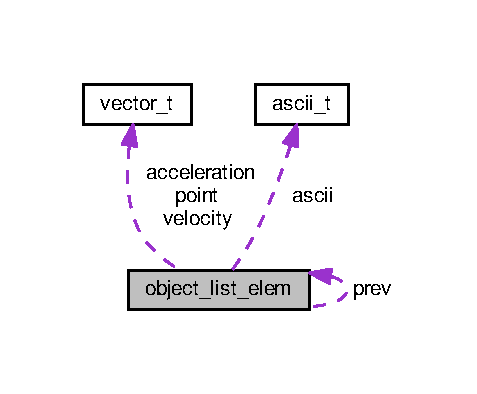
\includegraphics[width=229pt]{structobject__list__elem__coll__graph}
\end{center}
\end{figure}
\subsection*{Data Fields}
\begin{DoxyCompactItemize}
\item 
\hyperlink{object__list_8h_adee610a3c7375031538811d29f6a4124}{type\+\_\+t} \hyperlink{structobject__list__elem_aa84efc5c7fcf3887328cce7dc72fda67}{type}
\item 
\hyperlink{structvector__t}{vector\+\_\+t} \hyperlink{structobject__list__elem_a5e2e6e97dc9763c6713838d6f36fa0ba}{point}
\item 
\hyperlink{structvector__t}{vector\+\_\+t} \hyperlink{structobject__list__elem_affba049401aaf1488ce02106158a6b4b}{velocity}
\item 
\hyperlink{structvector__t}{vector\+\_\+t} \hyperlink{structobject__list__elem_a5bd8bb21c8d8b0d7b86e10773617ad55}{acceleration}
\item 
\hyperlink{structascii__t}{ascii\+\_\+t} $\ast$ \hyperlink{structobject__list__elem_ab490a018acd1306da39712322fa48597}{ascii}
\item 
uint16\+\_\+t \hyperlink{structobject__list__elem_ae5eb9e7b299437926de262dcc70de47e}{depth}
\item 
struct \hyperlink{structobject__list__elem}{object\+\_\+list\+\_\+elem} $\ast$ \hyperlink{structobject__list__elem_a71a54270804fe79669e899752f3e2992}{prev}
\end{DoxyCompactItemize}


\subsection{Detailed Description}
A struct to store the state of an object. 

\subsection{Field Documentation}
\index{object\+\_\+list\+\_\+elem@{object\+\_\+list\+\_\+elem}!acceleration@{acceleration}}
\index{acceleration@{acceleration}!object\+\_\+list\+\_\+elem@{object\+\_\+list\+\_\+elem}}
\subsubsection[{\texorpdfstring{acceleration}{acceleration}}]{\setlength{\rightskip}{0pt plus 5cm}{\bf vector\+\_\+t} object\+\_\+list\+\_\+elem\+::acceleration}\hypertarget{structobject__list__elem_a5bd8bb21c8d8b0d7b86e10773617ad55}{}\label{structobject__list__elem_a5bd8bb21c8d8b0d7b86e10773617ad55}
Acceleration of the object. \index{object\+\_\+list\+\_\+elem@{object\+\_\+list\+\_\+elem}!ascii@{ascii}}
\index{ascii@{ascii}!object\+\_\+list\+\_\+elem@{object\+\_\+list\+\_\+elem}}
\subsubsection[{\texorpdfstring{ascii}{ascii}}]{\setlength{\rightskip}{0pt plus 5cm}{\bf ascii\+\_\+t}$\ast$ object\+\_\+list\+\_\+elem\+::ascii}\hypertarget{structobject__list__elem_ab490a018acd1306da39712322fa48597}{}\label{structobject__list__elem_ab490a018acd1306da39712322fa48597}
A pointer to an ascii struct. \index{object\+\_\+list\+\_\+elem@{object\+\_\+list\+\_\+elem}!depth@{depth}}
\index{depth@{depth}!object\+\_\+list\+\_\+elem@{object\+\_\+list\+\_\+elem}}
\subsubsection[{\texorpdfstring{depth}{depth}}]{\setlength{\rightskip}{0pt plus 5cm}uint16\+\_\+t object\+\_\+list\+\_\+elem\+::depth}\hypertarget{structobject__list__elem_ae5eb9e7b299437926de262dcc70de47e}{}\label{structobject__list__elem_ae5eb9e7b299437926de262dcc70de47e}
Depth of the object. \index{object\+\_\+list\+\_\+elem@{object\+\_\+list\+\_\+elem}!point@{point}}
\index{point@{point}!object\+\_\+list\+\_\+elem@{object\+\_\+list\+\_\+elem}}
\subsubsection[{\texorpdfstring{point}{point}}]{\setlength{\rightskip}{0pt plus 5cm}{\bf vector\+\_\+t} object\+\_\+list\+\_\+elem\+::point}\hypertarget{structobject__list__elem_a5e2e6e97dc9763c6713838d6f36fa0ba}{}\label{structobject__list__elem_a5e2e6e97dc9763c6713838d6f36fa0ba}
Position of the object. \index{object\+\_\+list\+\_\+elem@{object\+\_\+list\+\_\+elem}!prev@{prev}}
\index{prev@{prev}!object\+\_\+list\+\_\+elem@{object\+\_\+list\+\_\+elem}}
\subsubsection[{\texorpdfstring{prev}{prev}}]{\setlength{\rightskip}{0pt plus 5cm}struct {\bf object\+\_\+list\+\_\+elem}$\ast$ object\+\_\+list\+\_\+elem\+::prev}\hypertarget{structobject__list__elem_a71a54270804fe79669e899752f3e2992}{}\label{structobject__list__elem_a71a54270804fe79669e899752f3e2992}
Previous object (used in snake). \index{object\+\_\+list\+\_\+elem@{object\+\_\+list\+\_\+elem}!type@{type}}
\index{type@{type}!object\+\_\+list\+\_\+elem@{object\+\_\+list\+\_\+elem}}
\subsubsection[{\texorpdfstring{type}{type}}]{\setlength{\rightskip}{0pt plus 5cm}{\bf type\+\_\+t} object\+\_\+list\+\_\+elem\+::type}\hypertarget{structobject__list__elem_aa84efc5c7fcf3887328cce7dc72fda67}{}\label{structobject__list__elem_aa84efc5c7fcf3887328cce7dc72fda67}
Type of the object. \index{object\+\_\+list\+\_\+elem@{object\+\_\+list\+\_\+elem}!velocity@{velocity}}
\index{velocity@{velocity}!object\+\_\+list\+\_\+elem@{object\+\_\+list\+\_\+elem}}
\subsubsection[{\texorpdfstring{velocity}{velocity}}]{\setlength{\rightskip}{0pt plus 5cm}{\bf vector\+\_\+t} object\+\_\+list\+\_\+elem\+::velocity}\hypertarget{structobject__list__elem_affba049401aaf1488ce02106158a6b4b}{}\label{structobject__list__elem_affba049401aaf1488ce02106158a6b4b}
Velocity of the object. 

The documentation for this struct was generated from the following file\+:\begin{DoxyCompactItemize}
\item 
flappy-\/bird/\hyperlink{object__list_8h}{object\+\_\+list.\+h}\end{DoxyCompactItemize}

\hypertarget{structobject__list__elem__t}{}\section{object\+\_\+list\+\_\+elem\+\_\+t Struct Reference}
\label{structobject__list__elem__t}\index{object\+\_\+list\+\_\+elem\+\_\+t@{object\+\_\+list\+\_\+elem\+\_\+t}}


Collaboration diagram for object\+\_\+list\+\_\+elem\+\_\+t\+:\nopagebreak
\begin{figure}[H]
\begin{center}
\leavevmode
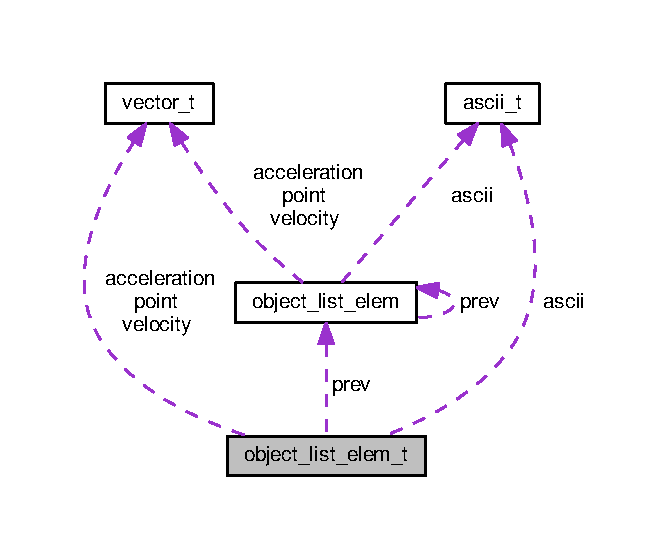
\includegraphics[width=322pt]{structobject__list__elem__t__coll__graph}
\end{center}
\end{figure}
\subsection*{Data Fields}
\begin{DoxyCompactItemize}
\item 
\hyperlink{object__list_8h_adee610a3c7375031538811d29f6a4124}{type\+\_\+t} {\bfseries type}\hypertarget{structobject__list__elem__t_a2a091e617e92fb4705dc37526803e93a}{}\label{structobject__list__elem__t_a2a091e617e92fb4705dc37526803e93a}

\item 
\hyperlink{structvector__t}{vector\+\_\+t} {\bfseries point}\hypertarget{structobject__list__elem__t_a22808567b3e124f69487e5405f6371fb}{}\label{structobject__list__elem__t_a22808567b3e124f69487e5405f6371fb}

\item 
\hyperlink{structvector__t}{vector\+\_\+t} {\bfseries velocity}\hypertarget{structobject__list__elem__t_a4addcc9c95c12d90c28adaf0b9a1a7a5}{}\label{structobject__list__elem__t_a4addcc9c95c12d90c28adaf0b9a1a7a5}

\item 
\hyperlink{structvector__t}{vector\+\_\+t} {\bfseries acceleration}\hypertarget{structobject__list__elem__t_afb9235562fcb2d64ca594de133237e4c}{}\label{structobject__list__elem__t_afb9235562fcb2d64ca594de133237e4c}

\item 
\hyperlink{structascii__t}{ascii\+\_\+t} $\ast$ {\bfseries ascii}\hypertarget{structobject__list__elem__t_a6cf92fc05b6904f73ed2a6d46a46bfcf}{}\label{structobject__list__elem__t_a6cf92fc05b6904f73ed2a6d46a46bfcf}

\item 
uint16\+\_\+t {\bfseries depth}\hypertarget{structobject__list__elem__t_a226f1ad4c575da7ea3853902c8eff9b7}{}\label{structobject__list__elem__t_a226f1ad4c575da7ea3853902c8eff9b7}

\item 
struct \hyperlink{structobject__list__elem}{object\+\_\+list\+\_\+elem} $\ast$ {\bfseries prev}\hypertarget{structobject__list__elem__t_a4008c76027a9e2e3e4eb34b205bc646b}{}\label{structobject__list__elem__t_a4008c76027a9e2e3e4eb34b205bc646b}

\end{DoxyCompactItemize}


The documentation for this struct was generated from the following file\+:\begin{DoxyCompactItemize}
\item 
flappy\+\_\+bird.\+c\end{DoxyCompactItemize}

\hypertarget{structobject__list__t}{}\section{object\+\_\+list\+\_\+t Struct Reference}
\label{structobject__list__t}\index{object\+\_\+list\+\_\+t@{object\+\_\+list\+\_\+t}}


A struct to store a list of objects.  




{\ttfamily \#include $<$object\+\_\+list.\+h$>$}



Collaboration diagram for object\+\_\+list\+\_\+t\+:\nopagebreak
\begin{figure}[H]
\begin{center}
\leavevmode
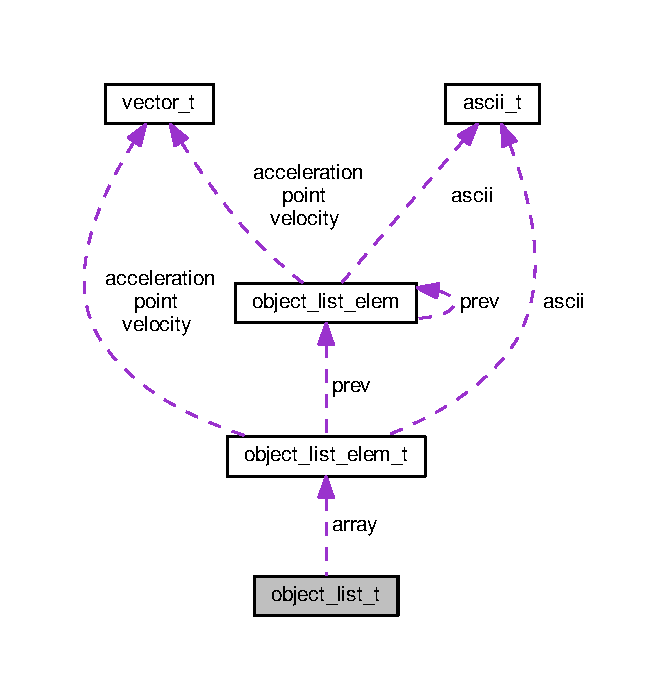
\includegraphics[width=322pt]{structobject__list__t__coll__graph}
\end{center}
\end{figure}
\subsection*{Data Fields}
\begin{DoxyCompactItemize}
\item 
\hyperlink{structobject__list__elem__t}{object\+\_\+list\+\_\+elem\+\_\+t} $\ast$$\ast$ \hyperlink{structobject__list__t_ab19231a7f3b4249002106ac152822819}{array}
\item 
uint16\+\_\+t \hyperlink{structobject__list__t_af656fe571a2562c31ae1ac9ebd4d7e79}{size}
\item 
uint16\+\_\+t \hyperlink{structobject__list__t_a577a0a7f314f10c0ffdd911f8b5a45f3}{max\+\_\+size}
\end{DoxyCompactItemize}


\subsection{Detailed Description}
A struct to store a list of objects. 

\subsection{Field Documentation}
\index{object\+\_\+list\+\_\+t@{object\+\_\+list\+\_\+t}!array@{array}}
\index{array@{array}!object\+\_\+list\+\_\+t@{object\+\_\+list\+\_\+t}}
\subsubsection[{\texorpdfstring{array}{array}}]{\setlength{\rightskip}{0pt plus 5cm}{\bf object\+\_\+list\+\_\+elem\+\_\+t} $\ast$$\ast$ object\+\_\+list\+\_\+t\+::array}\hypertarget{structobject__list__t_ab19231a7f3b4249002106ac152822819}{}\label{structobject__list__t_ab19231a7f3b4249002106ac152822819}
Array of pointers to objects. \index{object\+\_\+list\+\_\+t@{object\+\_\+list\+\_\+t}!max\+\_\+size@{max\+\_\+size}}
\index{max\+\_\+size@{max\+\_\+size}!object\+\_\+list\+\_\+t@{object\+\_\+list\+\_\+t}}
\subsubsection[{\texorpdfstring{max\+\_\+size}{max_size}}]{\setlength{\rightskip}{0pt plus 5cm}uint16\+\_\+t object\+\_\+list\+\_\+t\+::max\+\_\+size}\hypertarget{structobject__list__t_a577a0a7f314f10c0ffdd911f8b5a45f3}{}\label{structobject__list__t_a577a0a7f314f10c0ffdd911f8b5a45f3}
Size currently allocated for the array. \index{object\+\_\+list\+\_\+t@{object\+\_\+list\+\_\+t}!size@{size}}
\index{size@{size}!object\+\_\+list\+\_\+t@{object\+\_\+list\+\_\+t}}
\subsubsection[{\texorpdfstring{size}{size}}]{\setlength{\rightskip}{0pt plus 5cm}uint16\+\_\+t object\+\_\+list\+\_\+t\+::size}\hypertarget{structobject__list__t_af656fe571a2562c31ae1ac9ebd4d7e79}{}\label{structobject__list__t_af656fe571a2562c31ae1ac9ebd4d7e79}
Size of the array. 

The documentation for this struct was generated from the following files\+:\begin{DoxyCompactItemize}
\item 
flappy-\/bird/\hyperlink{object__list_8h}{object\+\_\+list.\+h}\item 
flappy\+\_\+bird.\+c\end{DoxyCompactItemize}

\hypertarget{structuchar__array__t}{}\section{uchar\+\_\+array\+\_\+t Struct Reference}
\label{structuchar__array__t}\index{uchar\+\_\+array\+\_\+t@{uchar\+\_\+array\+\_\+t}}


A struct to hold a unsigned char array. Also holds the size, and the standard deviation.  


\subsection*{Data Fields}
\begin{DoxyCompactItemize}
\item 
unsigned char $\ast$ \hyperlink{structuchar__array__t_a76655383d2ec294a6eb01685b3a72703}{array}
\item 
double \hyperlink{structuchar__array__t_a6debbe8b5be99042683abaae9961c91d}{standard\+\_\+dev}
\item 
int \hyperlink{structuchar__array__t_a7295f3a1d13730521639d49098861c60}{size}
\end{DoxyCompactItemize}


\subsection{Detailed Description}
A struct to hold a unsigned char array. Also holds the size, and the standard deviation. 

\subsection{Field Documentation}
\index{uchar\+\_\+array\+\_\+t@{uchar\+\_\+array\+\_\+t}!array@{array}}
\index{array@{array}!uchar\+\_\+array\+\_\+t@{uchar\+\_\+array\+\_\+t}}
\subsubsection[{\texorpdfstring{array}{array}}]{\setlength{\rightskip}{0pt plus 5cm}unsigned char$\ast$ uchar\+\_\+array\+\_\+t\+::array}\hypertarget{structuchar__array__t_a76655383d2ec294a6eb01685b3a72703}{}\label{structuchar__array__t_a76655383d2ec294a6eb01685b3a72703}
The unsigned char array. \index{uchar\+\_\+array\+\_\+t@{uchar\+\_\+array\+\_\+t}!size@{size}}
\index{size@{size}!uchar\+\_\+array\+\_\+t@{uchar\+\_\+array\+\_\+t}}
\subsubsection[{\texorpdfstring{size}{size}}]{\setlength{\rightskip}{0pt plus 5cm}int uchar\+\_\+array\+\_\+t\+::size}\hypertarget{structuchar__array__t_a7295f3a1d13730521639d49098861c60}{}\label{structuchar__array__t_a7295f3a1d13730521639d49098861c60}
The number of elements in the unsigned char array. \index{uchar\+\_\+array\+\_\+t@{uchar\+\_\+array\+\_\+t}!standard\+\_\+dev@{standard\+\_\+dev}}
\index{standard\+\_\+dev@{standard\+\_\+dev}!uchar\+\_\+array\+\_\+t@{uchar\+\_\+array\+\_\+t}}
\subsubsection[{\texorpdfstring{standard\+\_\+dev}{standard_dev}}]{\setlength{\rightskip}{0pt plus 5cm}double uchar\+\_\+array\+\_\+t\+::standard\+\_\+dev}\hypertarget{structuchar__array__t_a6debbe8b5be99042683abaae9961c91d}{}\label{structuchar__array__t_a6debbe8b5be99042683abaae9961c91d}
The standard deviation of the values in the unsigned char array. 

The documentation for this struct was generated from the following file\+:\begin{DoxyCompactItemize}
\item 
\hyperlink{uchar__array_8c}{uchar\+\_\+array.\+c}\end{DoxyCompactItemize}

\hypertarget{structvector__t}{}\section{vector\+\_\+t Struct Reference}
\label{structvector__t}\index{vector\+\_\+t@{vector\+\_\+t}}


A vector pair struct.  




{\ttfamily \#include $<$object\+\_\+list.\+h$>$}

\subsection*{Data Fields}
\begin{DoxyCompactItemize}
\item 
int16\+\_\+t \hyperlink{structvector__t_aaba677025136684726ba9652391b94fc}{x}
\item 
int16\+\_\+t \hyperlink{structvector__t_a0bca3dc392c2c1940205980ecfda1260}{y}
\end{DoxyCompactItemize}


\subsection{Detailed Description}
A vector pair struct. 

\subsection{Field Documentation}
\index{vector\+\_\+t@{vector\+\_\+t}!x@{x}}
\index{x@{x}!vector\+\_\+t@{vector\+\_\+t}}
\subsubsection[{\texorpdfstring{x}{x}}]{\setlength{\rightskip}{0pt plus 5cm}int16\+\_\+t vector\+\_\+t\+::x}\hypertarget{structvector__t_aaba677025136684726ba9652391b94fc}{}\label{structvector__t_aaba677025136684726ba9652391b94fc}
X value. \index{vector\+\_\+t@{vector\+\_\+t}!y@{y}}
\index{y@{y}!vector\+\_\+t@{vector\+\_\+t}}
\subsubsection[{\texorpdfstring{y}{y}}]{\setlength{\rightskip}{0pt plus 5cm}int16\+\_\+t vector\+\_\+t\+::y}\hypertarget{structvector__t_a0bca3dc392c2c1940205980ecfda1260}{}\label{structvector__t_a0bca3dc392c2c1940205980ecfda1260}
Y value. 

The documentation for this struct was generated from the following files\+:\begin{DoxyCompactItemize}
\item 
flappy-\/bird/\hyperlink{object__list_8h}{object\+\_\+list.\+h}\item 
flappy\+\_\+bird.\+c\end{DoxyCompactItemize}

\chapter{File Documentation}
\hypertarget{calibration_8c}{}\section{calibration.\+c File Reference}
\label{calibration_8c}\index{calibration.\+c@{calibration.\+c}}


Functions to calibrate colours.  


This graph shows which files directly or indirectly include this file\+:\nopagebreak
\begin{figure}[H]
\begin{center}
\leavevmode
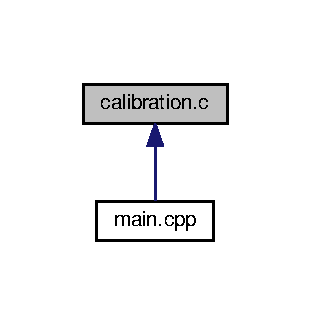
\includegraphics[width=149pt]{calibration_8c__dep__incl}
\end{center}
\end{figure}
\subsection*{Data Structures}
\begin{DoxyCompactItemize}
\item 
struct \hyperlink{structcalibration__t}{calibration\+\_\+t}
\begin{DoxyCompactList}\small\item\em A struct to hold the H\+SV values of the calibrated skin colour. \end{DoxyCompactList}\end{DoxyCompactItemize}
\subsection*{Functions}
\begin{DoxyCompactItemize}
\item 
bool \hyperlink{calibration_8c_ae5a332876fef43161febb75fb1355c8a}{in\+\_\+box} (int x, int y, int box\+\_\+x, int box\+\_\+y, int width, int height)
\begin{DoxyCompactList}\small\item\em Given a coordinate and a box, determines whether it is in the box. \end{DoxyCompactList}\item 
void \hyperlink{calibration_8c_aed953b3b59e6d4cb091a040919649956}{overlay\+\_\+frame} (Ipl\+Image $\ast$frame, int reg\+\_\+x, int reg\+\_\+y, int reg\+\_\+height, int reg\+\_\+width)
\begin{DoxyCompactList}\small\item\em Given a frame, applies a darkened border around it. User will place their hand inside the undarkened centre box to calibrate their skin colour. \end{DoxyCompactList}\item 
void \hyperlink{calibration_8c_aceafe429ab393d7f133fa456ea7d97b1}{final\+\_\+calibration} (Ipl\+Image $\ast$frame, \hyperlink{structcalibration__t}{calibration\+\_\+t} $\ast$c, int reg\+\_\+x, int reg\+\_\+y, int reg\+\_\+height, int reg\+\_\+width)
\begin{DoxyCompactList}\small\item\em Calibrates according to the skin colour in centre box in the frame. \end{DoxyCompactList}\item 
void \hyperlink{calibration_8c_ad1efc29c01e46f3615ba22fdbf7d5e02}{generic\+\_\+calibration} (\hyperlink{structcalibration__t}{calibration\+\_\+t} $\ast$c)
\begin{DoxyCompactList}\small\item\em Calibrates according to a generic skin colour. \end{DoxyCompactList}\item 
void \hyperlink{calibration_8c_a799f54885674567fe534511576edb9dc}{calibrate} (Cv\+Capture $\ast$capture, \hyperlink{structcalibration__t}{calibration\+\_\+t} $\ast$calibration)
\begin{DoxyCompactList}\small\item\em Displays a calibration window for the user to calibrate their skin. \end{DoxyCompactList}\end{DoxyCompactItemize}


\subsection{Detailed Description}
Functions to calibrate colours. 



\subsection{Function Documentation}
\index{calibration.\+c@{calibration.\+c}!calibrate@{calibrate}}
\index{calibrate@{calibrate}!calibration.\+c@{calibration.\+c}}
\subsubsection[{\texorpdfstring{calibrate(\+Cv\+Capture $\ast$capture, calibration\+\_\+t $\ast$calibration)}{calibrate(CvCapture *capture, calibration_t *calibration)}}]{\setlength{\rightskip}{0pt plus 5cm}void calibrate (
\begin{DoxyParamCaption}
\item[{Cv\+Capture $\ast$}]{capture, }
\item[{{\bf calibration\+\_\+t} $\ast$}]{calibration}
\end{DoxyParamCaption}
)}\hypertarget{calibration_8c_a799f54885674567fe534511576edb9dc}{}\label{calibration_8c_a799f54885674567fe534511576edb9dc}


Displays a calibration window for the user to calibrate their skin. 


\begin{DoxyParams}{Parameters}
{\em capture} & The Cv\+Capture video stream. \\
\hline
{\em calibration} & The calibration struct to place the skin colour values in. \\
\hline
\end{DoxyParams}
\index{calibration.\+c@{calibration.\+c}!final\+\_\+calibration@{final\+\_\+calibration}}
\index{final\+\_\+calibration@{final\+\_\+calibration}!calibration.\+c@{calibration.\+c}}
\subsubsection[{\texorpdfstring{final\+\_\+calibration(\+Ipl\+Image $\ast$frame, calibration\+\_\+t $\ast$c, int reg\+\_\+x, int reg\+\_\+y, int reg\+\_\+height, int reg\+\_\+width)}{final_calibration(IplImage *frame, calibration_t *c, int reg_x, int reg_y, int reg_height, int reg_width)}}]{\setlength{\rightskip}{0pt plus 5cm}void final\+\_\+calibration (
\begin{DoxyParamCaption}
\item[{Ipl\+Image $\ast$}]{frame, }
\item[{{\bf calibration\+\_\+t} $\ast$}]{c, }
\item[{int}]{reg\+\_\+x, }
\item[{int}]{reg\+\_\+y, }
\item[{int}]{reg\+\_\+height, }
\item[{int}]{reg\+\_\+width}
\end{DoxyParamCaption}
)}\hypertarget{calibration_8c_aceafe429ab393d7f133fa456ea7d97b1}{}\label{calibration_8c_aceafe429ab393d7f133fa456ea7d97b1}


Calibrates according to the skin colour in centre box in the frame. 


\begin{DoxyParams}{Parameters}
{\em frame} & The Ipl\+Image frame. \\
\hline
{\em c} & The calibration struct to place the skin colour values in. \\
\hline
{\em reg\+\_\+x} & The centre box x coordinate. \\
\hline
{\em reg\+\_\+y} & The centre box y coordinate. \\
\hline
{\em reg\+\_\+height} & The centre box height. \\
\hline
{\em reg\+\_\+width} & The centre box width. \\
\hline
\end{DoxyParams}
\index{calibration.\+c@{calibration.\+c}!generic\+\_\+calibration@{generic\+\_\+calibration}}
\index{generic\+\_\+calibration@{generic\+\_\+calibration}!calibration.\+c@{calibration.\+c}}
\subsubsection[{\texorpdfstring{generic\+\_\+calibration(calibration\+\_\+t $\ast$c)}{generic_calibration(calibration_t *c)}}]{\setlength{\rightskip}{0pt plus 5cm}void generic\+\_\+calibration (
\begin{DoxyParamCaption}
\item[{{\bf calibration\+\_\+t} $\ast$}]{c}
\end{DoxyParamCaption}
)}\hypertarget{calibration_8c_ad1efc29c01e46f3615ba22fdbf7d5e02}{}\label{calibration_8c_ad1efc29c01e46f3615ba22fdbf7d5e02}


Calibrates according to a generic skin colour. 


\begin{DoxyParams}{Parameters}
{\em c} & The calibration struct to place the skin colour values in. \\
\hline
\end{DoxyParams}
\index{calibration.\+c@{calibration.\+c}!in\+\_\+box@{in\+\_\+box}}
\index{in\+\_\+box@{in\+\_\+box}!calibration.\+c@{calibration.\+c}}
\subsubsection[{\texorpdfstring{in\+\_\+box(int x, int y, int box\+\_\+x, int box\+\_\+y, int width, int height)}{in_box(int x, int y, int box_x, int box_y, int width, int height)}}]{\setlength{\rightskip}{0pt plus 5cm}bool in\+\_\+box (
\begin{DoxyParamCaption}
\item[{int}]{x, }
\item[{int}]{y, }
\item[{int}]{box\+\_\+x, }
\item[{int}]{box\+\_\+y, }
\item[{int}]{width, }
\item[{int}]{height}
\end{DoxyParamCaption}
)}\hypertarget{calibration_8c_ae5a332876fef43161febb75fb1355c8a}{}\label{calibration_8c_ae5a332876fef43161febb75fb1355c8a}


Given a coordinate and a box, determines whether it is in the box. 


\begin{DoxyParams}{Parameters}
{\em x} & The x coordinate. \\
\hline
{\em y} & The y coordinate. \\
\hline
{\em box\+\_\+x} & The x coordinate of the centre of box. \\
\hline
{\em box\+\_\+y} & The y coordinate of the centre of box. \\
\hline
{\em width} & The distance from centre of the box to left or right edge. \\
\hline
{\em height} & The distance from centre of the box to top or bottom edge. \\
\hline
\end{DoxyParams}
\begin{DoxyReturn}{Returns}
True iff the coordinate is in the box. 
\end{DoxyReturn}
\index{calibration.\+c@{calibration.\+c}!overlay\+\_\+frame@{overlay\+\_\+frame}}
\index{overlay\+\_\+frame@{overlay\+\_\+frame}!calibration.\+c@{calibration.\+c}}
\subsubsection[{\texorpdfstring{overlay\+\_\+frame(\+Ipl\+Image $\ast$frame, int reg\+\_\+x, int reg\+\_\+y, int reg\+\_\+height, int reg\+\_\+width)}{overlay_frame(IplImage *frame, int reg_x, int reg_y, int reg_height, int reg_width)}}]{\setlength{\rightskip}{0pt plus 5cm}void overlay\+\_\+frame (
\begin{DoxyParamCaption}
\item[{Ipl\+Image $\ast$}]{frame, }
\item[{int}]{reg\+\_\+x, }
\item[{int}]{reg\+\_\+y, }
\item[{int}]{reg\+\_\+height, }
\item[{int}]{reg\+\_\+width}
\end{DoxyParamCaption}
)}\hypertarget{calibration_8c_aed953b3b59e6d4cb091a040919649956}{}\label{calibration_8c_aed953b3b59e6d4cb091a040919649956}


Given a frame, applies a darkened border around it. User will place their hand inside the undarkened centre box to calibrate their skin colour. 


\begin{DoxyParams}{Parameters}
{\em frame} & The Ipl\+Image frame. \\
\hline
{\em reg\+\_\+x} & The centre box x coordinate. \\
\hline
{\em reg\+\_\+y} & The centre box y coordinate. \\
\hline
{\em reg\+\_\+height} & The centre box height. \\
\hline
{\em reg\+\_\+width} & The centre box width. \\
\hline
\end{DoxyParams}

\hypertarget{detection_8c}{}\section{detection.\+c File Reference}
\label{detection_8c}\index{detection.\+c@{detection.\+c}}


Functions to detect position of hands.  


This graph shows which files directly or indirectly include this file\+:\nopagebreak
\begin{figure}[H]
\begin{center}
\leavevmode
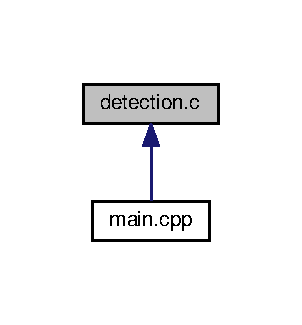
\includegraphics[width=145pt]{detection_8c__dep__incl}
\end{center}
\end{figure}
\subsection*{Data Structures}
\begin{DoxyCompactItemize}
\item 
struct \hyperlink{structhands__t}{hands\+\_\+t}
\begin{DoxyCompactList}\small\item\em A struct that holds information about the positions of hands. \end{DoxyCompactList}\end{DoxyCompactItemize}
\subsection*{Macros}
\begin{DoxyCompactItemize}
\item 
\#define {\bfseries I\+T\+E\+R\+A\+T\+I\+O\+NS}~10\hypertarget{detection_8c_aa9cc087d076e4fa101f8794a947bd01a}{}\label{detection_8c_aa9cc087d076e4fa101f8794a947bd01a}

\end{DoxyCompactItemize}
\subsection*{Functions}
\begin{DoxyCompactItemize}
\item 
\hyperlink{structhands__t}{hands\+\_\+t} $\ast$ \hyperlink{detection_8c_a02948972554282f1ea76afef45f735c7}{init\+\_\+hands} (void)
\begin{DoxyCompactList}\small\item\em Initialises the \hyperlink{structhands__t}{hands\+\_\+t} struct. \end{DoxyCompactList}\item 
double \hyperlink{detection_8c_a13e2aa455e1cc7d01751c4b4a35dc053}{dist} (int x, int y, int ux, int uy)
\begin{DoxyCompactList}\small\item\em Calculates distance between 2 points. \end{DoxyCompactList}\item 
void \hyperlink{detection_8c_ad4d12900f9017f74024a6ba1970998f7}{apply\+\_\+force\+\_\+point} (Ipl\+Image $\ast$frame, int $\ast$px, int $\ast$py, double initial, double scale)
\begin{DoxyCompactList}\small\item\em Applies forces to a single point, converging it to the users hand. \end{DoxyCompactList}\item 
void \hyperlink{detection_8c_a8816cbf0eb1257798bf51f4824039dc7}{apply\+\_\+force} (Ipl\+Image $\ast$frame, \hyperlink{structhands__t}{hands\+\_\+t} $\ast$h, double scale)
\begin{DoxyCompactList}\small\item\em Applies forces to left and right hand points. \end{DoxyCompactList}\item 
bool \hyperlink{detection_8c_aff9533b8dd99376fca5e19285ade1074}{outside\+\_\+range} (int x, int y, int rx, int ry, int rwidth, int rheight)
\begin{DoxyCompactList}\small\item\em Calculates if a point is outside a region. \end{DoxyCompactList}\item 
void \hyperlink{detection_8c_a82612834137e9eef986ce7f604aaef59}{detect\+\_\+hands} (Ipl\+Image $\ast$frame, \hyperlink{structhands__t}{hands\+\_\+t} $\ast$hands)
\begin{DoxyCompactList}\small\item\em Detects new positions of the users hands. \end{DoxyCompactList}\end{DoxyCompactItemize}


\subsection{Detailed Description}
Functions to detect position of hands. 



\subsection{Function Documentation}
\index{detection.\+c@{detection.\+c}!apply\+\_\+force@{apply\+\_\+force}}
\index{apply\+\_\+force@{apply\+\_\+force}!detection.\+c@{detection.\+c}}
\subsubsection[{\texorpdfstring{apply\+\_\+force(\+Ipl\+Image $\ast$frame, hands\+\_\+t $\ast$h, double scale)}{apply_force(IplImage *frame, hands_t *h, double scale)}}]{\setlength{\rightskip}{0pt plus 5cm}void apply\+\_\+force (
\begin{DoxyParamCaption}
\item[{Ipl\+Image $\ast$}]{frame, }
\item[{{\bf hands\+\_\+t} $\ast$}]{h, }
\item[{double}]{scale}
\end{DoxyParamCaption}
)}\hypertarget{detection_8c_a8816cbf0eb1257798bf51f4824039dc7}{}\label{detection_8c_a8816cbf0eb1257798bf51f4824039dc7}


Applies forces to left and right hand points. 


\begin{DoxyParams}{Parameters}
{\em frame} & The webcam image. \\
\hline
{\em h} & The hands struct to update. \\
\hline
{\em scale} & Scaling for how much the point moves. \\
\hline
\end{DoxyParams}
\index{detection.\+c@{detection.\+c}!apply\+\_\+force\+\_\+point@{apply\+\_\+force\+\_\+point}}
\index{apply\+\_\+force\+\_\+point@{apply\+\_\+force\+\_\+point}!detection.\+c@{detection.\+c}}
\subsubsection[{\texorpdfstring{apply\+\_\+force\+\_\+point(\+Ipl\+Image $\ast$frame, int $\ast$px, int $\ast$py, double initial, double scale)}{apply_force_point(IplImage *frame, int *px, int *py, double initial, double scale)}}]{\setlength{\rightskip}{0pt plus 5cm}void apply\+\_\+force\+\_\+point (
\begin{DoxyParamCaption}
\item[{Ipl\+Image $\ast$}]{frame, }
\item[{int $\ast$}]{px, }
\item[{int $\ast$}]{py, }
\item[{double}]{initial, }
\item[{double}]{scale}
\end{DoxyParamCaption}
)}\hypertarget{detection_8c_ad4d12900f9017f74024a6ba1970998f7}{}\label{detection_8c_ad4d12900f9017f74024a6ba1970998f7}


Applies forces to a single point, converging it to the users hand. 


\begin{DoxyParams}{Parameters}
{\em frame} & The webcam image. \\
\hline
{\em px} & A pointer to the x position of the point. \\
\hline
{\em py} & A pointer to the y position of the point. \\
\hline
{\em initial} & The initial x force to apply to the point. \\
\hline
{\em scale} & Scaling for how much the point moves. \\
\hline
\end{DoxyParams}
\index{detection.\+c@{detection.\+c}!detect\+\_\+hands@{detect\+\_\+hands}}
\index{detect\+\_\+hands@{detect\+\_\+hands}!detection.\+c@{detection.\+c}}
\subsubsection[{\texorpdfstring{detect\+\_\+hands(\+Ipl\+Image $\ast$frame, hands\+\_\+t $\ast$hands)}{detect_hands(IplImage *frame, hands_t *hands)}}]{\setlength{\rightskip}{0pt plus 5cm}void detect\+\_\+hands (
\begin{DoxyParamCaption}
\item[{Ipl\+Image $\ast$}]{frame, }
\item[{{\bf hands\+\_\+t} $\ast$}]{hands}
\end{DoxyParamCaption}
)}\hypertarget{detection_8c_a82612834137e9eef986ce7f604aaef59}{}\label{detection_8c_a82612834137e9eef986ce7f604aaef59}


Detects new positions of the users hands. 


\begin{DoxyParams}{Parameters}
{\em frame} & The newest webcam frame. \\
\hline
{\em hands} & The last position of the hands, is updated to be the new position. \\
\hline
\end{DoxyParams}
\index{detection.\+c@{detection.\+c}!dist@{dist}}
\index{dist@{dist}!detection.\+c@{detection.\+c}}
\subsubsection[{\texorpdfstring{dist(int x, int y, int ux, int uy)}{dist(int x, int y, int ux, int uy)}}]{\setlength{\rightskip}{0pt plus 5cm}double dist (
\begin{DoxyParamCaption}
\item[{int}]{x, }
\item[{int}]{y, }
\item[{int}]{ux, }
\item[{int}]{uy}
\end{DoxyParamCaption}
)}\hypertarget{detection_8c_a13e2aa455e1cc7d01751c4b4a35dc053}{}\label{detection_8c_a13e2aa455e1cc7d01751c4b4a35dc053}


Calculates distance between 2 points. 


\begin{DoxyParams}{Parameters}
{\em x} & x position of point1. \\
\hline
{\em y} & y position of point1. \\
\hline
{\em ux} & x position of point2. \\
\hline
{\em uy} & y position of point2. \\
\hline
\end{DoxyParams}
\begin{DoxyReturn}{Returns}
The distance between the 2 points. 
\end{DoxyReturn}
\index{detection.\+c@{detection.\+c}!init\+\_\+hands@{init\+\_\+hands}}
\index{init\+\_\+hands@{init\+\_\+hands}!detection.\+c@{detection.\+c}}
\subsubsection[{\texorpdfstring{init\+\_\+hands(void)}{init_hands(void)}}]{\setlength{\rightskip}{0pt plus 5cm}{\bf hands\+\_\+t}$\ast$ init\+\_\+hands (
\begin{DoxyParamCaption}
\item[{void}]{}
\end{DoxyParamCaption}
)}\hypertarget{detection_8c_a02948972554282f1ea76afef45f735c7}{}\label{detection_8c_a02948972554282f1ea76afef45f735c7}


Initialises the \hyperlink{structhands__t}{hands\+\_\+t} struct. 

\begin{DoxyReturn}{Returns}
A pointer to the new \hyperlink{structhands__t}{hands\+\_\+t} struct. 
\end{DoxyReturn}
\index{detection.\+c@{detection.\+c}!outside\+\_\+range@{outside\+\_\+range}}
\index{outside\+\_\+range@{outside\+\_\+range}!detection.\+c@{detection.\+c}}
\subsubsection[{\texorpdfstring{outside\+\_\+range(int x, int y, int rx, int ry, int rwidth, int rheight)}{outside_range(int x, int y, int rx, int ry, int rwidth, int rheight)}}]{\setlength{\rightskip}{0pt plus 5cm}bool outside\+\_\+range (
\begin{DoxyParamCaption}
\item[{int}]{x, }
\item[{int}]{y, }
\item[{int}]{rx, }
\item[{int}]{ry, }
\item[{int}]{rwidth, }
\item[{int}]{rheight}
\end{DoxyParamCaption}
)}\hypertarget{detection_8c_aff9533b8dd99376fca5e19285ade1074}{}\label{detection_8c_aff9533b8dd99376fca5e19285ade1074}


Calculates if a point is outside a region. 


\begin{DoxyParams}{Parameters}
{\em x} & X pos of the point. \\
\hline
{\em y} & Y pos of the point. \\
\hline
{\em rx} & X pos of the region. \\
\hline
{\em ry} & Y pos of the region. \\
\hline
{\em rwidth} & Width of the region. \\
\hline
{\em rheight} & Height of the region. \\
\hline
\end{DoxyParams}
\begin{DoxyReturn}{Returns}
true if the point is outside the region, false otherwise. 
\end{DoxyReturn}

\hypertarget{ascii__art_8h}{}\section{flappy-\/bird/ascii\+\_\+art.h File Reference}
\label{ascii__art_8h}\index{flappy-\/bird/ascii\+\_\+art.\+h@{flappy-\/bird/ascii\+\_\+art.\+h}}


Header to define the \hyperlink{structascii__t}{ascii\+\_\+t} struct.  


{\ttfamily \#include $<$stdint.\+h$>$}\\*
Include dependency graph for ascii\+\_\+art.\+h\+:\nopagebreak
\begin{figure}[H]
\begin{center}
\leavevmode
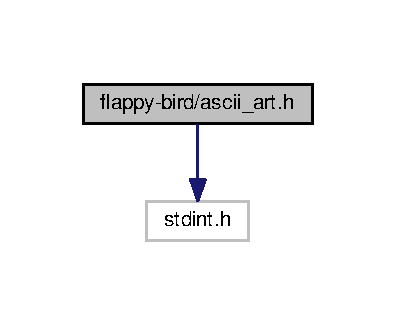
\includegraphics[width=190pt]{ascii__art_8h__incl}
\end{center}
\end{figure}
This graph shows which files directly or indirectly include this file\+:\nopagebreak
\begin{figure}[H]
\begin{center}
\leavevmode
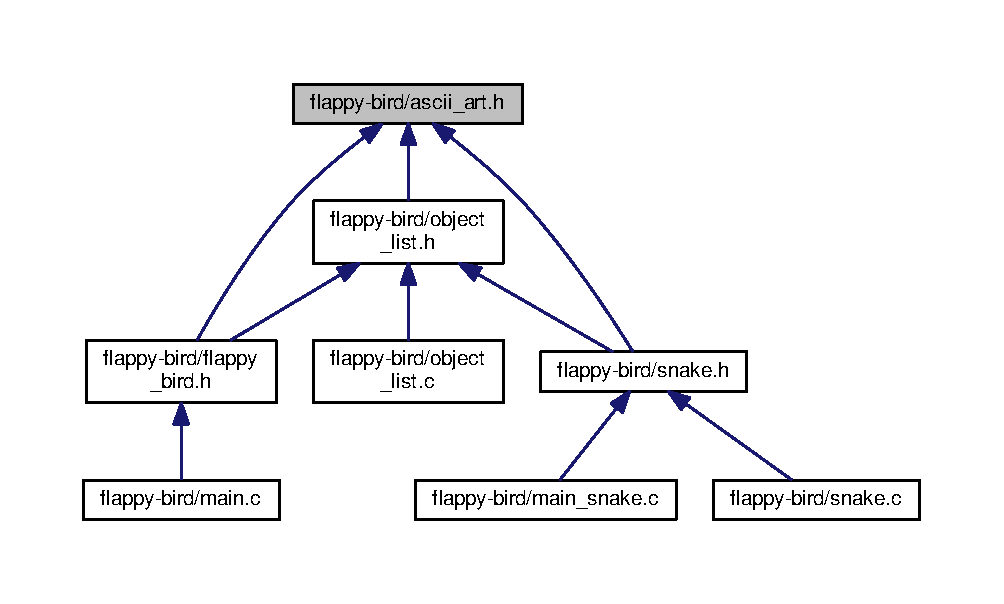
\includegraphics[width=350pt]{ascii__art_8h__dep__incl}
\end{center}
\end{figure}
\subsection*{Data Structures}
\begin{DoxyCompactItemize}
\item 
struct \hyperlink{structascii__t}{ascii\+\_\+t}
\begin{DoxyCompactList}\small\item\em A struct to hold information about an A\+S\+C\+II sprite. \end{DoxyCompactList}\end{DoxyCompactItemize}
\subsection*{Macros}
\begin{DoxyCompactItemize}
\item 
\#define \hyperlink{ascii__art_8h_ae48f170084a4c2e566805bbc084afbed}{E\+M\+P\+T\+Y\+\_\+\+S\+P\+A\+CE}~\textquotesingle{} \textquotesingle{}
\end{DoxyCompactItemize}


\subsection{Detailed Description}
Header to define the \hyperlink{structascii__t}{ascii\+\_\+t} struct. 



\subsection{Macro Definition Documentation}
\index{ascii\+\_\+art.\+h@{ascii\+\_\+art.\+h}!E\+M\+P\+T\+Y\+\_\+\+S\+P\+A\+CE@{E\+M\+P\+T\+Y\+\_\+\+S\+P\+A\+CE}}
\index{E\+M\+P\+T\+Y\+\_\+\+S\+P\+A\+CE@{E\+M\+P\+T\+Y\+\_\+\+S\+P\+A\+CE}!ascii\+\_\+art.\+h@{ascii\+\_\+art.\+h}}
\subsubsection[{\texorpdfstring{E\+M\+P\+T\+Y\+\_\+\+S\+P\+A\+CE}{EMPTY_SPACE}}]{\setlength{\rightskip}{0pt plus 5cm}\#define E\+M\+P\+T\+Y\+\_\+\+S\+P\+A\+CE~\textquotesingle{} \textquotesingle{}}\hypertarget{ascii__art_8h_ae48f170084a4c2e566805bbc084afbed}{}\label{ascii__art_8h_ae48f170084a4c2e566805bbc084afbed}
Defines a blank character for use in A\+S\+C\+II output. 
\hypertarget{flappy__bird_8h}{}\section{flappy-\/bird/flappy\+\_\+bird.h File Reference}
\label{flappy__bird_8h}\index{flappy-\/bird/flappy\+\_\+bird.\+h@{flappy-\/bird/flappy\+\_\+bird.\+h}}


Header file for flappy bird.  


{\ttfamily \#include $<$stdio.\+h$>$}\\*
{\ttfamily \#include $<$stdlib.\+h$>$}\\*
{\ttfamily \#include $<$unistd.\+h$>$}\\*
{\ttfamily \#include $<$time.\+h$>$}\\*
{\ttfamily \#include $<$ncurses.\+h$>$}\\*
{\ttfamily \#include \char`\"{}ascii\+\_\+art.\+h\char`\"{}}\\*
{\ttfamily \#include \char`\"{}object\+\_\+list.\+h\char`\"{}}\\*
{\ttfamily \#include $<$locale.\+h$>$}\\*
Include dependency graph for flappy\+\_\+bird.\+h\+:\nopagebreak
\begin{figure}[H]
\begin{center}
\leavevmode
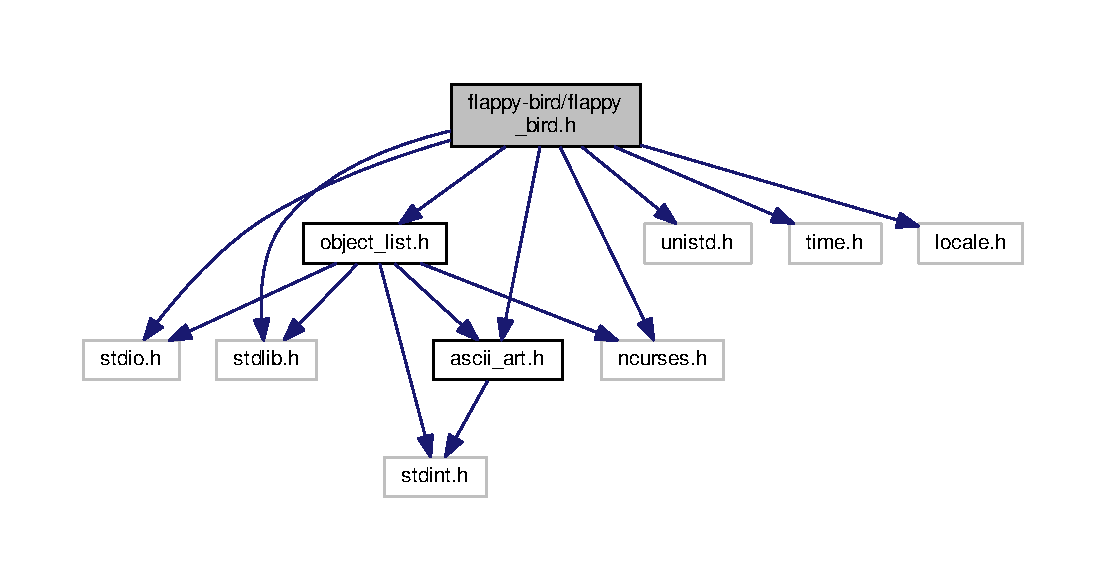
\includegraphics[width=350pt]{flappy__bird_8h__incl}
\end{center}
\end{figure}
This graph shows which files directly or indirectly include this file\+:\nopagebreak
\begin{figure}[H]
\begin{center}
\leavevmode
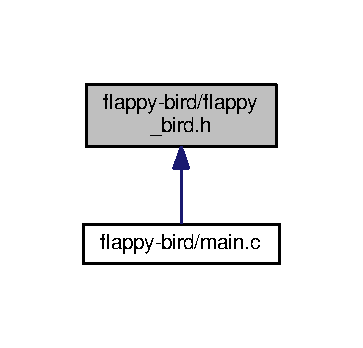
\includegraphics[width=174pt]{flappy__bird_8h__dep__incl}
\end{center}
\end{figure}
\subsection*{Macros}
\begin{DoxyCompactItemize}
\item 
\#define \hyperlink{flappy__bird_8h_a241aeeb764887ae5e3de58b98f04b16d}{W\+I\+D\+TH}~300
\item 
\#define \hyperlink{flappy__bird_8h_aed89bd71aee8be823e8a20ec4e093c1e}{H\+E\+I\+G\+HT}~100
\end{DoxyCompactItemize}
\subsection*{Functions}
\begin{DoxyCompactItemize}
\item 
void \hyperlink{flappy__bird_8h_a3b902613461225bf63bce5edba6ffc41}{move\+\_\+pipes} (\hyperlink{structobject__list__elem__t}{object\+\_\+list\+\_\+elem\+\_\+t} $\ast$elem)
\begin{DoxyCompactList}\small\item\em Moves pipes that go off the screen to come back again. \end{DoxyCompactList}\item 
void \hyperlink{flappy__bird_8h_af4eb214e10d7aaeab2154492b26ce34e}{flap} (\hyperlink{structobject__list__elem__t}{object\+\_\+list\+\_\+elem\+\_\+t} $\ast$elem)
\begin{DoxyCompactList}\small\item\em Flaps the bird. \end{DoxyCompactList}\item 
int \hyperlink{flappy__bird_8h_a7f50b187387b6a10fffae9ed5809f741}{bird\+\_\+coll} (\hyperlink{structobject__list__t}{object\+\_\+list\+\_\+t} $\ast$list)
\begin{DoxyCompactList}\small\item\em Returns if the bird is dead or alive. \end{DoxyCompactList}\item 
\hyperlink{structobject__list__t}{object\+\_\+list\+\_\+t} $\ast$ \hyperlink{flappy__bird_8h_a762b57e20d9c7f2d75f7c67f72e839cf}{init\+\_\+game} (void)
\begin{DoxyCompactList}\small\item\em Initailises a game state for a flappy bird game. \end{DoxyCompactList}\item 
void \hyperlink{flappy__bird_8h_a73eabc67ee2946d88d6a855f1db5ef2b}{render\+\_\+game} (\hyperlink{structobject__list__t}{object\+\_\+list\+\_\+t} $\ast$list)
\begin{DoxyCompactList}\small\item\em Renders the game, and updates the game state. \end{DoxyCompactList}\end{DoxyCompactItemize}


\subsection{Detailed Description}
Header file for flappy bird. 



\subsection{Macro Definition Documentation}
\index{flappy\+\_\+bird.\+h@{flappy\+\_\+bird.\+h}!H\+E\+I\+G\+HT@{H\+E\+I\+G\+HT}}
\index{H\+E\+I\+G\+HT@{H\+E\+I\+G\+HT}!flappy\+\_\+bird.\+h@{flappy\+\_\+bird.\+h}}
\subsubsection[{\texorpdfstring{H\+E\+I\+G\+HT}{HEIGHT}}]{\setlength{\rightskip}{0pt plus 5cm}\#define H\+E\+I\+G\+HT~100}\hypertarget{flappy__bird_8h_aed89bd71aee8be823e8a20ec4e093c1e}{}\label{flappy__bird_8h_aed89bd71aee8be823e8a20ec4e093c1e}
Height of the game, in characters. \index{flappy\+\_\+bird.\+h@{flappy\+\_\+bird.\+h}!W\+I\+D\+TH@{W\+I\+D\+TH}}
\index{W\+I\+D\+TH@{W\+I\+D\+TH}!flappy\+\_\+bird.\+h@{flappy\+\_\+bird.\+h}}
\subsubsection[{\texorpdfstring{W\+I\+D\+TH}{WIDTH}}]{\setlength{\rightskip}{0pt plus 5cm}\#define W\+I\+D\+TH~300}\hypertarget{flappy__bird_8h_a241aeeb764887ae5e3de58b98f04b16d}{}\label{flappy__bird_8h_a241aeeb764887ae5e3de58b98f04b16d}
Width of the game, in characters. 

\subsection{Function Documentation}
\index{flappy\+\_\+bird.\+h@{flappy\+\_\+bird.\+h}!bird\+\_\+coll@{bird\+\_\+coll}}
\index{bird\+\_\+coll@{bird\+\_\+coll}!flappy\+\_\+bird.\+h@{flappy\+\_\+bird.\+h}}
\subsubsection[{\texorpdfstring{bird\+\_\+coll(object\+\_\+list\+\_\+t $\ast$list)}{bird_coll(object_list_t *list)}}]{\setlength{\rightskip}{0pt plus 5cm}int bird\+\_\+coll (
\begin{DoxyParamCaption}
\item[{{\bf object\+\_\+list\+\_\+t} $\ast$}]{list}
\end{DoxyParamCaption}
)}\hypertarget{flappy__bird_8h_a7f50b187387b6a10fffae9ed5809f741}{}\label{flappy__bird_8h_a7f50b187387b6a10fffae9ed5809f741}


Returns if the bird is dead or alive. 


\begin{DoxyParams}{Parameters}
{\em list} & The object list.  0 if the bird is alive, 1 otherwise. \\
\hline
\end{DoxyParams}
\index{flappy\+\_\+bird.\+h@{flappy\+\_\+bird.\+h}!flap@{flap}}
\index{flap@{flap}!flappy\+\_\+bird.\+h@{flappy\+\_\+bird.\+h}}
\subsubsection[{\texorpdfstring{flap(object\+\_\+list\+\_\+elem\+\_\+t $\ast$elem)}{flap(object_list_elem_t *elem)}}]{\setlength{\rightskip}{0pt plus 5cm}void flap (
\begin{DoxyParamCaption}
\item[{{\bf object\+\_\+list\+\_\+elem\+\_\+t} $\ast$}]{elem}
\end{DoxyParamCaption}
)}\hypertarget{flappy__bird_8h_af4eb214e10d7aaeab2154492b26ce34e}{}\label{flappy__bird_8h_af4eb214e10d7aaeab2154492b26ce34e}


Flaps the bird. 

Is a object\+\_\+list\+\_\+elem\+\_\+function\+\_\+t so can be called with for\+\_\+all. 
\begin{DoxyParams}{Parameters}
{\em elem} & Object to move. \\
\hline
\end{DoxyParams}
\index{flappy\+\_\+bird.\+h@{flappy\+\_\+bird.\+h}!init\+\_\+game@{init\+\_\+game}}
\index{init\+\_\+game@{init\+\_\+game}!flappy\+\_\+bird.\+h@{flappy\+\_\+bird.\+h}}
\subsubsection[{\texorpdfstring{init\+\_\+game(void)}{init_game(void)}}]{\setlength{\rightskip}{0pt plus 5cm}{\bf object\+\_\+list\+\_\+t}$\ast$ init\+\_\+game (
\begin{DoxyParamCaption}
\item[{void}]{}
\end{DoxyParamCaption}
)}\hypertarget{flappy__bird_8h_a762b57e20d9c7f2d75f7c67f72e839cf}{}\label{flappy__bird_8h_a762b57e20d9c7f2d75f7c67f72e839cf}


Initailises a game state for a flappy bird game. 

\begin{DoxyReturn}{Returns}
An object list representing the initial game state.
\end{DoxyReturn}
Initailises a game state for a flappy bird game.

\begin{DoxyReturn}{Returns}
An object list representing the initial game state. 
\end{DoxyReturn}
\index{flappy\+\_\+bird.\+h@{flappy\+\_\+bird.\+h}!move\+\_\+pipes@{move\+\_\+pipes}}
\index{move\+\_\+pipes@{move\+\_\+pipes}!flappy\+\_\+bird.\+h@{flappy\+\_\+bird.\+h}}
\subsubsection[{\texorpdfstring{move\+\_\+pipes(object\+\_\+list\+\_\+elem\+\_\+t $\ast$elem)}{move_pipes(object_list_elem_t *elem)}}]{\setlength{\rightskip}{0pt plus 5cm}void move\+\_\+pipes (
\begin{DoxyParamCaption}
\item[{{\bf object\+\_\+list\+\_\+elem\+\_\+t} $\ast$}]{elem}
\end{DoxyParamCaption}
)}\hypertarget{flappy__bird_8h_a3b902613461225bf63bce5edba6ffc41}{}\label{flappy__bird_8h_a3b902613461225bf63bce5edba6ffc41}


Moves pipes that go off the screen to come back again. 

Is a object\+\_\+list\+\_\+elem\+\_\+function\+\_\+t so can be called with for\+\_\+all. 
\begin{DoxyParams}{Parameters}
{\em elem} & Object to move. \\
\hline
\end{DoxyParams}
\index{flappy\+\_\+bird.\+h@{flappy\+\_\+bird.\+h}!render\+\_\+game@{render\+\_\+game}}
\index{render\+\_\+game@{render\+\_\+game}!flappy\+\_\+bird.\+h@{flappy\+\_\+bird.\+h}}
\subsubsection[{\texorpdfstring{render\+\_\+game(object\+\_\+list\+\_\+t $\ast$list)}{render_game(object_list_t *list)}}]{\setlength{\rightskip}{0pt plus 5cm}void render\+\_\+game (
\begin{DoxyParamCaption}
\item[{{\bf object\+\_\+list\+\_\+t} $\ast$}]{list}
\end{DoxyParamCaption}
)}\hypertarget{flappy__bird_8h_a73eabc67ee2946d88d6a855f1db5ef2b}{}\label{flappy__bird_8h_a73eabc67ee2946d88d6a855f1db5ef2b}


Renders the game, and updates the game state. 


\begin{DoxyParams}{Parameters}
{\em list} & The object list. \\
\hline
\end{DoxyParams}

\hypertarget{main_8c}{}\section{flappy-\/bird/main.c File Reference}
\label{main_8c}\index{flappy-\/bird/main.\+c@{flappy-\/bird/main.\+c}}


Main file for flappy bird game.  


{\ttfamily \#include \char`\"{}flappy\+\_\+bird.\+h\char`\"{}}\\*
Include dependency graph for main.\+c\+:\nopagebreak
\begin{figure}[H]
\begin{center}
\leavevmode
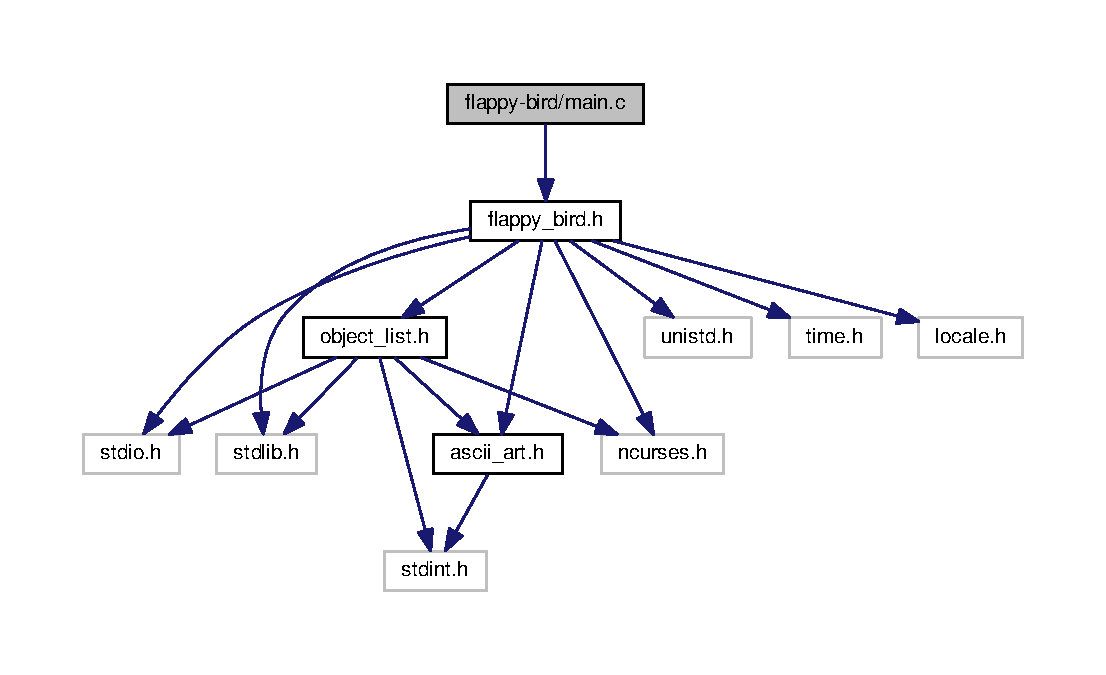
\includegraphics[width=350pt]{main_8c__incl}
\end{center}
\end{figure}
\subsection*{Functions}
\begin{DoxyCompactItemize}
\item 
int \hyperlink{main_8c_a3c04138a5bfe5d72780bb7e82a18e627}{main} (int argc, char $\ast$$\ast$argv)\hypertarget{main_8c_a3c04138a5bfe5d72780bb7e82a18e627}{}\label{main_8c_a3c04138a5bfe5d72780bb7e82a18e627}

\begin{DoxyCompactList}\small\item\em Makes and plays the game, space bar controls. \end{DoxyCompactList}\end{DoxyCompactItemize}


\subsection{Detailed Description}
Main file for flappy bird game. 


\hypertarget{main__snake_8c}{}\section{flappy-\/bird/main\+\_\+snake.c File Reference}
\label{main__snake_8c}\index{flappy-\/bird/main\+\_\+snake.\+c@{flappy-\/bird/main\+\_\+snake.\+c}}


Main file for snake game.  


{\ttfamily \#include \char`\"{}snake.\+h\char`\"{}}\\*
Include dependency graph for main\+\_\+snake.\+c\+:\nopagebreak
\begin{figure}[H]
\begin{center}
\leavevmode
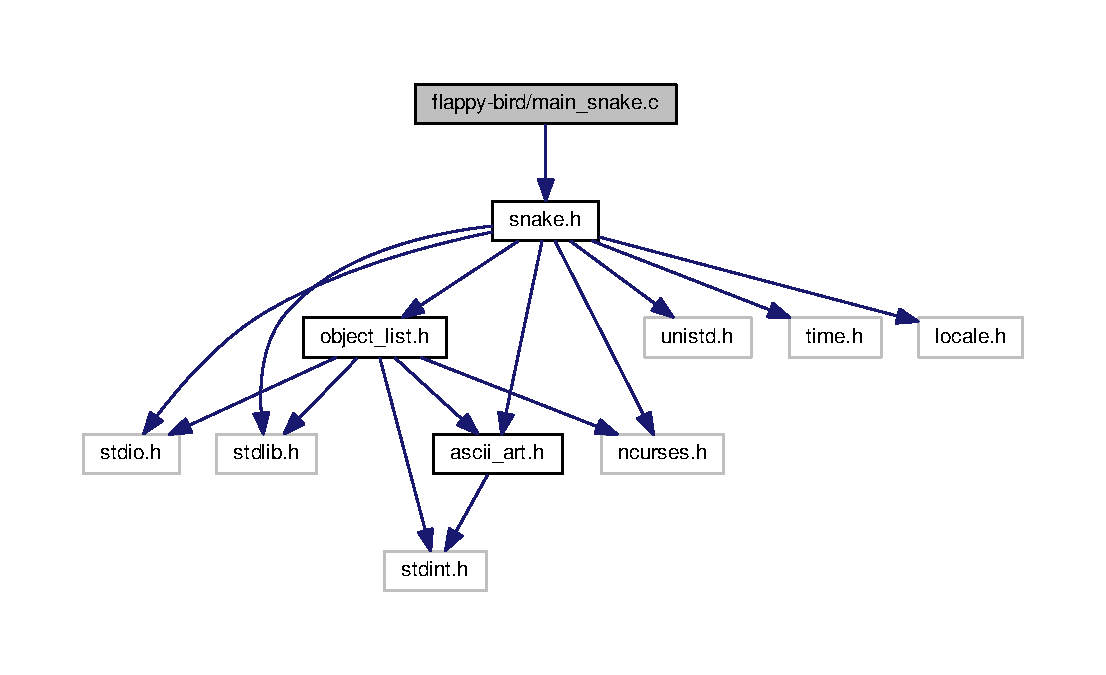
\includegraphics[width=350pt]{main__snake_8c__incl}
\end{center}
\end{figure}
\subsection*{Functions}
\begin{DoxyCompactItemize}
\item 
int \hyperlink{main__snake_8c_a840291bc02cba5474a4cb46a9b9566fe}{main} (void)\hypertarget{main__snake_8c_a840291bc02cba5474a4cb46a9b9566fe}{}\label{main__snake_8c_a840291bc02cba5474a4cb46a9b9566fe}

\begin{DoxyCompactList}\small\item\em Creates and plays the game, W\+A\+SD controls. \end{DoxyCompactList}\end{DoxyCompactItemize}


\subsection{Detailed Description}
Main file for snake game. 


\hypertarget{object__list_8c}{}\section{flappy-\/bird/object\+\_\+list.c File Reference}
\label{object__list_8c}\index{flappy-\/bird/object\+\_\+list.\+c@{flappy-\/bird/object\+\_\+list.\+c}}


Functions for using object list.  


{\ttfamily \#include \char`\"{}object\+\_\+list.\+h\char`\"{}}\\*
Include dependency graph for object\+\_\+list.\+c\+:\nopagebreak
\begin{figure}[H]
\begin{center}
\leavevmode
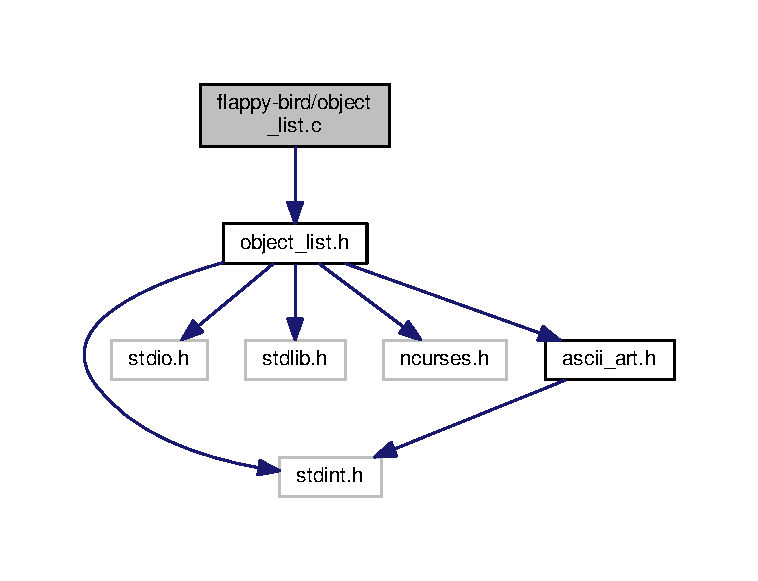
\includegraphics[width=350pt]{object__list_8c__incl}
\end{center}
\end{figure}
\subsection*{Functions}
\begin{DoxyCompactItemize}
\item 
\hyperlink{structobject__list__t}{object\+\_\+list\+\_\+t} $\ast$ \hyperlink{object__list_8c_aae6290424084da7690cb865db2d0e862}{new\+\_\+list} (void)
\begin{DoxyCompactList}\small\item\em Returns an initialised object list. \end{DoxyCompactList}\item 
void \hyperlink{object__list_8c_aa9ac729f1918ea527a60e5a769468d6f}{add\+\_\+elem} (\hyperlink{structobject__list__t}{object\+\_\+list\+\_\+t} $\ast$list, \hyperlink{structobject__list__elem__t}{object\+\_\+list\+\_\+elem\+\_\+t} $\ast$elem)
\begin{DoxyCompactList}\small\item\em Adds a element to an object list. \end{DoxyCompactList}\item 
int \hyperlink{object__list_8c_a5dc17578dcc024c7a0565da1f09731ef}{is\+\_\+covering} (\hyperlink{structobject__list__elem__t}{object\+\_\+list\+\_\+elem\+\_\+t} $\ast$elem, \hyperlink{structvector__t}{vector\+\_\+t} point)
\begin{DoxyCompactList}\small\item\em Returns if the object is covering the point. \end{DoxyCompactList}\item 
char \hyperlink{object__list_8c_ab255cb4f59e0897d84e1fcd1f13d0aaf}{get\+\_\+char\+\_\+ascii} (\hyperlink{structascii__t}{ascii\+\_\+t} $\ast$ascii, \hyperlink{structvector__t}{vector\+\_\+t} point)
\begin{DoxyCompactList}\small\item\em Returns the char at a given position in the ascii ascii\+\_\+art. \end{DoxyCompactList}\item 
char \hyperlink{object__list_8c_a5717656aa7aaf47fbb157dea036caa64}{get\+\_\+char\+\_\+list} (\hyperlink{structobject__list__t}{object\+\_\+list\+\_\+t} $\ast$list, \hyperlink{structvector__t}{vector\+\_\+t} point)
\begin{DoxyCompactList}\small\item\em Returns the char at a given position. \end{DoxyCompactList}\item 
void \hyperlink{object__list_8c_a3e25de16af12613be7fd6af5352dd278}{for\+\_\+all} (\hyperlink{structobject__list__t}{object\+\_\+list\+\_\+t} $\ast$list, \hyperlink{object__list_8h_a8c0ae6099b8fdca0e67d9becdcf7f41a}{object\+\_\+list\+\_\+elem\+\_\+function\+\_\+t} function)
\begin{DoxyCompactList}\small\item\em Applies a function to a object list. \end{DoxyCompactList}\item 
void \hyperlink{object__list_8c_ae864a67817f9ab01b9dce31622db8bd4}{move\+\_\+object} (\hyperlink{structobject__list__elem__t}{object\+\_\+list\+\_\+elem\+\_\+t} $\ast$elem)
\begin{DoxyCompactList}\small\item\em Moves an object and updates its velocity. \end{DoxyCompactList}\item 
void \hyperlink{object__list_8c_ab1699f73a3d81de38bd9c257fd5c7c33}{print\+\_\+object} (\hyperlink{structobject__list__elem__t}{object\+\_\+list\+\_\+elem\+\_\+t} $\ast$elem)
\begin{DoxyCompactList}\small\item\em Prints out an object. \end{DoxyCompactList}\item 
\hyperlink{structobject__list__elem__t}{object\+\_\+list\+\_\+elem\+\_\+t} $\ast$ \hyperlink{object__list_8c_af3f2fc8910c4c511173818e9513d7e78}{get\+\_\+elem} (\hyperlink{structobject__list__t}{object\+\_\+list\+\_\+t} $\ast$list, \hyperlink{object__list_8h_adee610a3c7375031538811d29f6a4124}{type\+\_\+t} type)
\begin{DoxyCompactList}\small\item\em Gets the first element with a matching type in the list. \end{DoxyCompactList}\item 
int \hyperlink{object__list_8c_adfeca24f8c478e115ecbf3aea11d8ba7}{get\+\_\+color} (\hyperlink{structobject__list__t}{object\+\_\+list\+\_\+t} $\ast$list, \hyperlink{structvector__t}{vector\+\_\+t} point)
\begin{DoxyCompactList}\small\item\em Returns the colour for a paticular position. \end{DoxyCompactList}\item 
void \hyperlink{object__list_8c_ade10433a1987f67f338680acedef6e37}{print\+\_\+game} (\hyperlink{structobject__list__t}{object\+\_\+list\+\_\+t} $\ast$list, int width, int height)
\begin{DoxyCompactList}\small\item\em Prints the game. \end{DoxyCompactList}\item 
void \hyperlink{object__list_8c_ad001d6c6eab89b13e3a3d3de8577a2a8}{free\+\_\+object\+\_\+list} (\hyperlink{structobject__list__t}{object\+\_\+list\+\_\+t} $\ast$list)
\begin{DoxyCompactList}\small\item\em Free\textquotesingle{}s all data used in the object list. \end{DoxyCompactList}\item 
void \hyperlink{object__list_8c_a49b883aa53db8bccee0f12c877ff35d8}{free\+\_\+object\+\_\+list\+\_\+elem} (\hyperlink{structobject__list__elem__t}{object\+\_\+list\+\_\+elem\+\_\+t} $\ast$elem)
\begin{DoxyCompactList}\small\item\em Frees an object. \end{DoxyCompactList}\end{DoxyCompactItemize}


\subsection{Detailed Description}
Functions for using object list. 



\subsection{Function Documentation}
\index{object\+\_\+list.\+c@{object\+\_\+list.\+c}!add\+\_\+elem@{add\+\_\+elem}}
\index{add\+\_\+elem@{add\+\_\+elem}!object\+\_\+list.\+c@{object\+\_\+list.\+c}}
\subsubsection[{\texorpdfstring{add\+\_\+elem(object\+\_\+list\+\_\+t $\ast$list, object\+\_\+list\+\_\+elem\+\_\+t $\ast$elem)}{add_elem(object_list_t *list, object_list_elem_t *elem)}}]{\setlength{\rightskip}{0pt plus 5cm}void add\+\_\+elem (
\begin{DoxyParamCaption}
\item[{{\bf object\+\_\+list\+\_\+t} $\ast$}]{list, }
\item[{{\bf object\+\_\+list\+\_\+elem\+\_\+t} $\ast$}]{elem}
\end{DoxyParamCaption}
)}\hypertarget{object__list_8c_aa9ac729f1918ea527a60e5a769468d6f}{}\label{object__list_8c_aa9ac729f1918ea527a60e5a769468d6f}


Adds a element to an object list. 


\begin{DoxyParams}{Parameters}
{\em list} & Object list to add element to. \\
\hline
{\em elem} & Object list elem to add to the list. \\
\hline
\end{DoxyParams}
\index{object\+\_\+list.\+c@{object\+\_\+list.\+c}!for\+\_\+all@{for\+\_\+all}}
\index{for\+\_\+all@{for\+\_\+all}!object\+\_\+list.\+c@{object\+\_\+list.\+c}}
\subsubsection[{\texorpdfstring{for\+\_\+all(object\+\_\+list\+\_\+t $\ast$list, object\+\_\+list\+\_\+elem\+\_\+function\+\_\+t function)}{for_all(object_list_t *list, object_list_elem_function_t function)}}]{\setlength{\rightskip}{0pt plus 5cm}void for\+\_\+all (
\begin{DoxyParamCaption}
\item[{{\bf object\+\_\+list\+\_\+t} $\ast$}]{list, }
\item[{{\bf object\+\_\+list\+\_\+elem\+\_\+function\+\_\+t}}]{function}
\end{DoxyParamCaption}
)}\hypertarget{object__list_8c_a3e25de16af12613be7fd6af5352dd278}{}\label{object__list_8c_a3e25de16af12613be7fd6af5352dd278}


Applies a function to a object list. 


\begin{DoxyParams}{Parameters}
{\em list} & Object list to apply the function to. \\
\hline
{\em function} & Function to apply. \\
\hline
\end{DoxyParams}
\index{object\+\_\+list.\+c@{object\+\_\+list.\+c}!free\+\_\+object\+\_\+list@{free\+\_\+object\+\_\+list}}
\index{free\+\_\+object\+\_\+list@{free\+\_\+object\+\_\+list}!object\+\_\+list.\+c@{object\+\_\+list.\+c}}
\subsubsection[{\texorpdfstring{free\+\_\+object\+\_\+list(object\+\_\+list\+\_\+t $\ast$list)}{free_object_list(object_list_t *list)}}]{\setlength{\rightskip}{0pt plus 5cm}void free\+\_\+object\+\_\+list (
\begin{DoxyParamCaption}
\item[{{\bf object\+\_\+list\+\_\+t} $\ast$}]{list}
\end{DoxyParamCaption}
)}\hypertarget{object__list_8c_ad001d6c6eab89b13e3a3d3de8577a2a8}{}\label{object__list_8c_ad001d6c6eab89b13e3a3d3de8577a2a8}


Free\textquotesingle{}s all data used in the object list. 


\begin{DoxyParams}{Parameters}
{\em list} & Object list to free. \\
\hline
\end{DoxyParams}
\index{object\+\_\+list.\+c@{object\+\_\+list.\+c}!free\+\_\+object\+\_\+list\+\_\+elem@{free\+\_\+object\+\_\+list\+\_\+elem}}
\index{free\+\_\+object\+\_\+list\+\_\+elem@{free\+\_\+object\+\_\+list\+\_\+elem}!object\+\_\+list.\+c@{object\+\_\+list.\+c}}
\subsubsection[{\texorpdfstring{free\+\_\+object\+\_\+list\+\_\+elem(object\+\_\+list\+\_\+elem\+\_\+t $\ast$elem)}{free_object_list_elem(object_list_elem_t *elem)}}]{\setlength{\rightskip}{0pt plus 5cm}void free\+\_\+object\+\_\+list\+\_\+elem (
\begin{DoxyParamCaption}
\item[{{\bf object\+\_\+list\+\_\+elem\+\_\+t} $\ast$}]{elem}
\end{DoxyParamCaption}
)}\hypertarget{object__list_8c_a49b883aa53db8bccee0f12c877ff35d8}{}\label{object__list_8c_a49b883aa53db8bccee0f12c877ff35d8}


Frees an object. 

Is a object\+\_\+list\+\_\+elem\+\_\+function\+\_\+t so can be called with for\+\_\+all. 
\begin{DoxyParams}{Parameters}
{\em elem} & Object to free. \\
\hline
\end{DoxyParams}
\index{object\+\_\+list.\+c@{object\+\_\+list.\+c}!get\+\_\+char\+\_\+ascii@{get\+\_\+char\+\_\+ascii}}
\index{get\+\_\+char\+\_\+ascii@{get\+\_\+char\+\_\+ascii}!object\+\_\+list.\+c@{object\+\_\+list.\+c}}
\subsubsection[{\texorpdfstring{get\+\_\+char\+\_\+ascii(ascii\+\_\+t $\ast$ascii, vector\+\_\+t point)}{get_char_ascii(ascii_t *ascii, vector_t point)}}]{\setlength{\rightskip}{0pt plus 5cm}char get\+\_\+char\+\_\+ascii (
\begin{DoxyParamCaption}
\item[{{\bf ascii\+\_\+t} $\ast$}]{ascii, }
\item[{{\bf vector\+\_\+t}}]{point}
\end{DoxyParamCaption}
)}\hypertarget{object__list_8c_ab255cb4f59e0897d84e1fcd1f13d0aaf}{}\label{object__list_8c_ab255cb4f59e0897d84e1fcd1f13d0aaf}


Returns the char at a given position in the ascii ascii\+\_\+art. 


\begin{DoxyParams}{Parameters}
{\em ascii} & A struct storing the ascii art. \\
\hline
{\em point} & Position in the ascii. \\
\hline
\end{DoxyParams}
\begin{DoxyReturn}{Returns}
Char at the position. 
\end{DoxyReturn}
\index{object\+\_\+list.\+c@{object\+\_\+list.\+c}!get\+\_\+char\+\_\+list@{get\+\_\+char\+\_\+list}}
\index{get\+\_\+char\+\_\+list@{get\+\_\+char\+\_\+list}!object\+\_\+list.\+c@{object\+\_\+list.\+c}}
\subsubsection[{\texorpdfstring{get\+\_\+char\+\_\+list(object\+\_\+list\+\_\+t $\ast$list, vector\+\_\+t point)}{get_char_list(object_list_t *list, vector_t point)}}]{\setlength{\rightskip}{0pt plus 5cm}char get\+\_\+char\+\_\+list (
\begin{DoxyParamCaption}
\item[{{\bf object\+\_\+list\+\_\+t} $\ast$}]{list, }
\item[{{\bf vector\+\_\+t}}]{point}
\end{DoxyParamCaption}
)}\hypertarget{object__list_8c_a5717656aa7aaf47fbb157dea036caa64}{}\label{object__list_8c_a5717656aa7aaf47fbb157dea036caa64}


Returns the char at a given position. 


\begin{DoxyParams}{Parameters}
{\em list} & Object list. \\
\hline
{\em point} & Position of the char. \\
\hline
\end{DoxyParams}
\begin{DoxyReturn}{Returns}
Char at given position. 
\end{DoxyReturn}
\index{object\+\_\+list.\+c@{object\+\_\+list.\+c}!get\+\_\+color@{get\+\_\+color}}
\index{get\+\_\+color@{get\+\_\+color}!object\+\_\+list.\+c@{object\+\_\+list.\+c}}
\subsubsection[{\texorpdfstring{get\+\_\+color(object\+\_\+list\+\_\+t $\ast$list, vector\+\_\+t point)}{get_color(object_list_t *list, vector_t point)}}]{\setlength{\rightskip}{0pt plus 5cm}int get\+\_\+color (
\begin{DoxyParamCaption}
\item[{{\bf object\+\_\+list\+\_\+t} $\ast$}]{list, }
\item[{{\bf vector\+\_\+t}}]{point}
\end{DoxyParamCaption}
)}\hypertarget{object__list_8c_adfeca24f8c478e115ecbf3aea11d8ba7}{}\label{object__list_8c_adfeca24f8c478e115ecbf3aea11d8ba7}


Returns the colour for a paticular position. 


\begin{DoxyParams}{Parameters}
{\em list} & The current game state. \\
\hline
{\em point} & The position to return the colour of. \\
\hline
\end{DoxyParams}
\begin{DoxyReturn}{Returns}
The colour of the position. 
\end{DoxyReturn}
\index{object\+\_\+list.\+c@{object\+\_\+list.\+c}!get\+\_\+elem@{get\+\_\+elem}}
\index{get\+\_\+elem@{get\+\_\+elem}!object\+\_\+list.\+c@{object\+\_\+list.\+c}}
\subsubsection[{\texorpdfstring{get\+\_\+elem(object\+\_\+list\+\_\+t $\ast$list, type\+\_\+t type)}{get_elem(object_list_t *list, type_t type)}}]{\setlength{\rightskip}{0pt plus 5cm}{\bf object\+\_\+list\+\_\+elem\+\_\+t} $\ast$ get\+\_\+elem (
\begin{DoxyParamCaption}
\item[{{\bf object\+\_\+list\+\_\+t} $\ast$}]{list, }
\item[{{\bf type\+\_\+t}}]{type}
\end{DoxyParamCaption}
)}\hypertarget{object__list_8c_af3f2fc8910c4c511173818e9513d7e78}{}\label{object__list_8c_af3f2fc8910c4c511173818e9513d7e78}


Gets the first element with a matching type in the list. 


\begin{DoxyParams}{Parameters}
{\em list} & List to look through. \\
\hline
{\em type} & Type of object to fine. \\
\hline
\end{DoxyParams}
\begin{DoxyReturn}{Returns}
Object with matching type. 
\end{DoxyReturn}
\index{object\+\_\+list.\+c@{object\+\_\+list.\+c}!is\+\_\+covering@{is\+\_\+covering}}
\index{is\+\_\+covering@{is\+\_\+covering}!object\+\_\+list.\+c@{object\+\_\+list.\+c}}
\subsubsection[{\texorpdfstring{is\+\_\+covering(object\+\_\+list\+\_\+elem\+\_\+t $\ast$elem, vector\+\_\+t point)}{is_covering(object_list_elem_t *elem, vector_t point)}}]{\setlength{\rightskip}{0pt plus 5cm}int is\+\_\+covering (
\begin{DoxyParamCaption}
\item[{{\bf object\+\_\+list\+\_\+elem\+\_\+t} $\ast$}]{elem, }
\item[{{\bf vector\+\_\+t}}]{point}
\end{DoxyParamCaption}
)}\hypertarget{object__list_8c_a5dc17578dcc024c7a0565da1f09731ef}{}\label{object__list_8c_a5dc17578dcc024c7a0565da1f09731ef}


Returns if the object is covering the point. 


\begin{DoxyParams}{Parameters}
{\em elem} & Object to check.  Position to check. \\
\hline
\end{DoxyParams}
\begin{DoxyReturn}{Returns}
1 if covering, 0 otherwise. 
\end{DoxyReturn}
\index{object\+\_\+list.\+c@{object\+\_\+list.\+c}!move\+\_\+object@{move\+\_\+object}}
\index{move\+\_\+object@{move\+\_\+object}!object\+\_\+list.\+c@{object\+\_\+list.\+c}}
\subsubsection[{\texorpdfstring{move\+\_\+object(object\+\_\+list\+\_\+elem\+\_\+t $\ast$elem)}{move_object(object_list_elem_t *elem)}}]{\setlength{\rightskip}{0pt plus 5cm}void move\+\_\+object (
\begin{DoxyParamCaption}
\item[{{\bf object\+\_\+list\+\_\+elem\+\_\+t} $\ast$}]{elem}
\end{DoxyParamCaption}
)}\hypertarget{object__list_8c_ae864a67817f9ab01b9dce31622db8bd4}{}\label{object__list_8c_ae864a67817f9ab01b9dce31622db8bd4}


Moves an object and updates its velocity. 

Is a object\+\_\+list\+\_\+elem\+\_\+function\+\_\+t so can be called with for\+\_\+all. 
\begin{DoxyParams}{Parameters}
{\em elem} & Object to move. \\
\hline
\end{DoxyParams}
\index{object\+\_\+list.\+c@{object\+\_\+list.\+c}!new\+\_\+list@{new\+\_\+list}}
\index{new\+\_\+list@{new\+\_\+list}!object\+\_\+list.\+c@{object\+\_\+list.\+c}}
\subsubsection[{\texorpdfstring{new\+\_\+list(void)}{new_list(void)}}]{\setlength{\rightskip}{0pt plus 5cm}{\bf object\+\_\+list\+\_\+t} $\ast$ new\+\_\+list (
\begin{DoxyParamCaption}
\item[{void}]{}
\end{DoxyParamCaption}
)}\hypertarget{object__list_8c_aae6290424084da7690cb865db2d0e862}{}\label{object__list_8c_aae6290424084da7690cb865db2d0e862}


Returns an initialised object list. 

\begin{DoxyReturn}{Returns}
Initialised object list. 
\end{DoxyReturn}
\index{object\+\_\+list.\+c@{object\+\_\+list.\+c}!print\+\_\+game@{print\+\_\+game}}
\index{print\+\_\+game@{print\+\_\+game}!object\+\_\+list.\+c@{object\+\_\+list.\+c}}
\subsubsection[{\texorpdfstring{print\+\_\+game(object\+\_\+list\+\_\+t $\ast$list, int width, int height)}{print_game(object_list_t *list, int width, int height)}}]{\setlength{\rightskip}{0pt plus 5cm}void print\+\_\+game (
\begin{DoxyParamCaption}
\item[{{\bf object\+\_\+list\+\_\+t} $\ast$}]{list, }
\item[{int}]{width, }
\item[{int}]{height}
\end{DoxyParamCaption}
)}\hypertarget{object__list_8c_ade10433a1987f67f338680acedef6e37}{}\label{object__list_8c_ade10433a1987f67f338680acedef6e37}


Prints the game. 


\begin{DoxyParams}{Parameters}
{\em list} & The current game state. \\
\hline
{\em width} & Width of the screen being used. \\
\hline
{\em height} & Height of the screen being used. \\
\hline
\end{DoxyParams}
\index{object\+\_\+list.\+c@{object\+\_\+list.\+c}!print\+\_\+object@{print\+\_\+object}}
\index{print\+\_\+object@{print\+\_\+object}!object\+\_\+list.\+c@{object\+\_\+list.\+c}}
\subsubsection[{\texorpdfstring{print\+\_\+object(object\+\_\+list\+\_\+elem\+\_\+t $\ast$elem)}{print_object(object_list_elem_t *elem)}}]{\setlength{\rightskip}{0pt plus 5cm}void print\+\_\+object (
\begin{DoxyParamCaption}
\item[{{\bf object\+\_\+list\+\_\+elem\+\_\+t} $\ast$}]{elem}
\end{DoxyParamCaption}
)}\hypertarget{object__list_8c_ab1699f73a3d81de38bd9c257fd5c7c33}{}\label{object__list_8c_ab1699f73a3d81de38bd9c257fd5c7c33}


Prints out an object. 

Is a object\+\_\+list\+\_\+elem\+\_\+function\+\_\+t so can be called with for\+\_\+all. 
\begin{DoxyParams}{Parameters}
{\em elem} & Object to print. \\
\hline
\end{DoxyParams}

\hypertarget{object__list_8h}{}\section{flappy-\/bird/object\+\_\+list.h File Reference}
\label{object__list_8h}\index{flappy-\/bird/object\+\_\+list.\+h@{flappy-\/bird/object\+\_\+list.\+h}}


Data type for storing the state of the game.  


{\ttfamily \#include $<$stdint.\+h$>$}\\*
{\ttfamily \#include $<$stdio.\+h$>$}\\*
{\ttfamily \#include $<$stdlib.\+h$>$}\\*
{\ttfamily \#include $<$ncurses.\+h$>$}\\*
{\ttfamily \#include \char`\"{}ascii\+\_\+art.\+h\char`\"{}}\\*
Include dependency graph for object\+\_\+list.\+h\+:\nopagebreak
\begin{figure}[H]
\begin{center}
\leavevmode
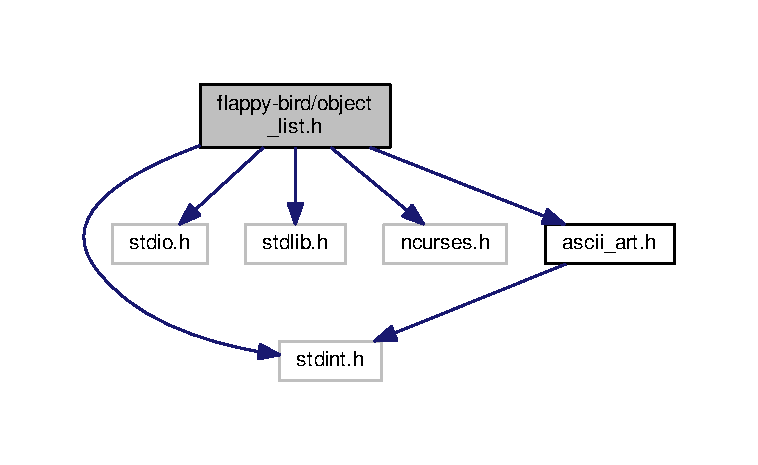
\includegraphics[width=350pt]{object__list_8h__incl}
\end{center}
\end{figure}
This graph shows which files directly or indirectly include this file\+:\nopagebreak
\begin{figure}[H]
\begin{center}
\leavevmode
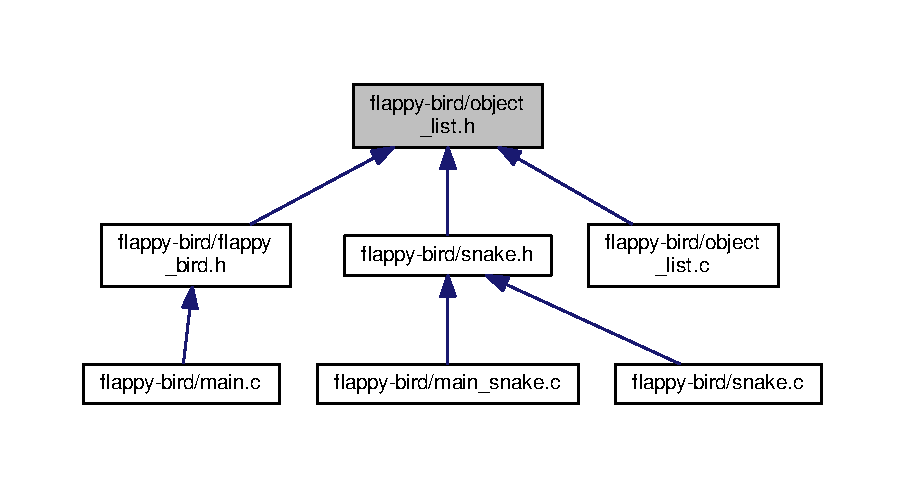
\includegraphics[width=350pt]{object__list_8h__dep__incl}
\end{center}
\end{figure}
\subsection*{Data Structures}
\begin{DoxyCompactItemize}
\item 
struct \hyperlink{structvector__t}{vector\+\_\+t}
\begin{DoxyCompactList}\small\item\em A vector pair struct. \end{DoxyCompactList}\item 
struct \hyperlink{structobject__list__elem}{object\+\_\+list\+\_\+elem}
\begin{DoxyCompactList}\small\item\em A struct to store the state of an object. \end{DoxyCompactList}\item 
struct \hyperlink{structobject__list__t}{object\+\_\+list\+\_\+t}
\begin{DoxyCompactList}\small\item\em A struct to store a list of objects. \end{DoxyCompactList}\end{DoxyCompactItemize}
\subsection*{Macros}
\begin{DoxyCompactItemize}
\item 
\#define \hyperlink{object__list_8h_a04b412d04e415d878767eab5ffff4677}{I\+N\+I\+T\+I\+A\+L\+\_\+\+O\+B\+J\+E\+C\+T\+\_\+\+L\+I\+S\+T\+\_\+\+S\+I\+ZE}~20
\end{DoxyCompactItemize}
\subsection*{Typedefs}
\begin{DoxyCompactItemize}
\item 
typedef struct \hyperlink{structobject__list__elem}{object\+\_\+list\+\_\+elem} \hyperlink{object__list_8h_aa7f60b410e6fda9534caeb8370a37afe}{object\+\_\+list\+\_\+elem\+\_\+t}\hypertarget{object__list_8h_aa7f60b410e6fda9534caeb8370a37afe}{}\label{object__list_8h_aa7f60b410e6fda9534caeb8370a37afe}

\begin{DoxyCompactList}\small\item\em A struct to store the state of an object. \end{DoxyCompactList}\item 
typedef void \hyperlink{object__list_8h_a8c0ae6099b8fdca0e67d9becdcf7f41a}{object\+\_\+list\+\_\+elem\+\_\+function\+\_\+t}(\hyperlink{structobject__list__elem__t}{object\+\_\+list\+\_\+elem\+\_\+t} $\ast$)
\end{DoxyCompactItemize}
\subsection*{Enumerations}
\begin{DoxyCompactItemize}
\item 
enum \hyperlink{object__list_8h_adee610a3c7375031538811d29f6a4124}{type\+\_\+t} \{ \\*
\hyperlink{object__list_8h_adee610a3c7375031538811d29f6a4124a2e5a1d1868aa44bc89666a660fbd80c1}{bird}, 
\hyperlink{object__list_8h_adee610a3c7375031538811d29f6a4124ae981b0996a25c6ce78fdcdeb2760fcb9}{pipes}, 
\hyperlink{object__list_8h_adee610a3c7375031538811d29f6a4124a8f8fb34d055a92cd148205c30448191d}{cloud}, 
\hyperlink{object__list_8h_adee610a3c7375031538811d29f6a4124a831e08074fc31bab018bf359a0184978}{ground}, 
\\*
\hyperlink{object__list_8h_adee610a3c7375031538811d29f6a4124a623729bc7f52fd9fe906d7419b6cb6a9}{snake\+\_\+head}, 
\hyperlink{object__list_8h_adee610a3c7375031538811d29f6a4124a4c042afd04f58519cd7423e6692bcb51}{snake\+\_\+body}, 
\hyperlink{object__list_8h_adee610a3c7375031538811d29f6a4124ae8d97019b10b7f38ac6111ce32bce9cb}{snake\+\_\+tail}, 
\hyperlink{object__list_8h_adee610a3c7375031538811d29f6a4124abd99b5b55239e844758c74c59b9e7d41}{snake\+\_\+apple}, 
\\*
{\bfseries bird}, 
{\bfseries pipes}, 
{\bfseries cloud}, 
{\bfseries ground}, 
\\*
{\bfseries snake\+\_\+head}, 
{\bfseries snake\+\_\+body}, 
{\bfseries snake\+\_\+tail}, 
{\bfseries snake\+\_\+apple}
 \}\begin{DoxyCompactList}\small\item\em An enum to store the type of the object. \end{DoxyCompactList}
\end{DoxyCompactItemize}
\subsection*{Functions}
\begin{DoxyCompactItemize}
\item 
\hyperlink{structobject__list__t}{object\+\_\+list\+\_\+t} $\ast$ \hyperlink{object__list_8h_aa07b767ecbf25d42522f5e5c6cfa162d}{new\+\_\+list} (void)
\begin{DoxyCompactList}\small\item\em Returns an initialised object list. \end{DoxyCompactList}\item 
void \hyperlink{object__list_8h_aa9ac729f1918ea527a60e5a769468d6f}{add\+\_\+elem} (\hyperlink{structobject__list__t}{object\+\_\+list\+\_\+t} $\ast$list, \hyperlink{structobject__list__elem__t}{object\+\_\+list\+\_\+elem\+\_\+t} $\ast$elem)
\begin{DoxyCompactList}\small\item\em Adds a element to an object list. \end{DoxyCompactList}\item 
int \hyperlink{object__list_8h_a5dc17578dcc024c7a0565da1f09731ef}{is\+\_\+covering} (\hyperlink{structobject__list__elem__t}{object\+\_\+list\+\_\+elem\+\_\+t} $\ast$elem, \hyperlink{structvector__t}{vector\+\_\+t} point)
\begin{DoxyCompactList}\small\item\em Returns if the object is covering the point. \end{DoxyCompactList}\item 
char \hyperlink{object__list_8h_ab255cb4f59e0897d84e1fcd1f13d0aaf}{get\+\_\+char\+\_\+ascii} (\hyperlink{structascii__t}{ascii\+\_\+t} $\ast$ascii, \hyperlink{structvector__t}{vector\+\_\+t} point)
\begin{DoxyCompactList}\small\item\em Returns the char at a given position in the ascii ascii\+\_\+art. \end{DoxyCompactList}\item 
char \hyperlink{object__list_8h_a5717656aa7aaf47fbb157dea036caa64}{get\+\_\+char\+\_\+list} (\hyperlink{structobject__list__t}{object\+\_\+list\+\_\+t} $\ast$list, \hyperlink{structvector__t}{vector\+\_\+t} point)
\begin{DoxyCompactList}\small\item\em Returns the char at a given position. \end{DoxyCompactList}\item 
void \hyperlink{object__list_8h_a3e25de16af12613be7fd6af5352dd278}{for\+\_\+all} (\hyperlink{structobject__list__t}{object\+\_\+list\+\_\+t} $\ast$list, \hyperlink{object__list_8h_a8c0ae6099b8fdca0e67d9becdcf7f41a}{object\+\_\+list\+\_\+elem\+\_\+function\+\_\+t} function)
\begin{DoxyCompactList}\small\item\em Applies a function to a object list. \end{DoxyCompactList}\item 
void \hyperlink{object__list_8h_ae864a67817f9ab01b9dce31622db8bd4}{move\+\_\+object} (\hyperlink{structobject__list__elem__t}{object\+\_\+list\+\_\+elem\+\_\+t} $\ast$elem)
\begin{DoxyCompactList}\small\item\em Moves an object and updates its velocity. \end{DoxyCompactList}\item 
void \hyperlink{object__list_8h_ab1699f73a3d81de38bd9c257fd5c7c33}{print\+\_\+object} (\hyperlink{structobject__list__elem__t}{object\+\_\+list\+\_\+elem\+\_\+t} $\ast$elem)
\begin{DoxyCompactList}\small\item\em Prints out an object. \end{DoxyCompactList}\item 
int \hyperlink{object__list_8h_adfeca24f8c478e115ecbf3aea11d8ba7}{get\+\_\+color} (\hyperlink{structobject__list__t}{object\+\_\+list\+\_\+t} $\ast$list, \hyperlink{structvector__t}{vector\+\_\+t} point)
\begin{DoxyCompactList}\small\item\em Returns the colour for a paticular position. \end{DoxyCompactList}\item 
void \hyperlink{object__list_8h_ade10433a1987f67f338680acedef6e37}{print\+\_\+game} (\hyperlink{structobject__list__t}{object\+\_\+list\+\_\+t} $\ast$list, int width, int height)
\begin{DoxyCompactList}\small\item\em Prints the game. \end{DoxyCompactList}\item 
void \hyperlink{object__list_8h_ad001d6c6eab89b13e3a3d3de8577a2a8}{free\+\_\+object\+\_\+list} (\hyperlink{structobject__list__t}{object\+\_\+list\+\_\+t} $\ast$list)
\begin{DoxyCompactList}\small\item\em Free\textquotesingle{}s all data used in the object list. \end{DoxyCompactList}\item 
void \hyperlink{object__list_8h_a49b883aa53db8bccee0f12c877ff35d8}{free\+\_\+object\+\_\+list\+\_\+elem} (\hyperlink{structobject__list__elem__t}{object\+\_\+list\+\_\+elem\+\_\+t} $\ast$elem)
\begin{DoxyCompactList}\small\item\em Frees an object. \end{DoxyCompactList}\item 
\hyperlink{structobject__list__elem__t}{object\+\_\+list\+\_\+elem\+\_\+t} $\ast$ \hyperlink{object__list_8h_af714066fdea3e60e3fa9f81aacba166a}{get\+\_\+elem} (\hyperlink{structobject__list__t}{object\+\_\+list\+\_\+t} $\ast$list, \hyperlink{object__list_8h_adee610a3c7375031538811d29f6a4124}{type\+\_\+t} type)
\begin{DoxyCompactList}\small\item\em Gets the first element with a matching type in the list. \end{DoxyCompactList}\end{DoxyCompactItemize}


\subsection{Detailed Description}
Data type for storing the state of the game. 



\subsection{Macro Definition Documentation}
\index{object\+\_\+list.\+h@{object\+\_\+list.\+h}!I\+N\+I\+T\+I\+A\+L\+\_\+\+O\+B\+J\+E\+C\+T\+\_\+\+L\+I\+S\+T\+\_\+\+S\+I\+ZE@{I\+N\+I\+T\+I\+A\+L\+\_\+\+O\+B\+J\+E\+C\+T\+\_\+\+L\+I\+S\+T\+\_\+\+S\+I\+ZE}}
\index{I\+N\+I\+T\+I\+A\+L\+\_\+\+O\+B\+J\+E\+C\+T\+\_\+\+L\+I\+S\+T\+\_\+\+S\+I\+ZE@{I\+N\+I\+T\+I\+A\+L\+\_\+\+O\+B\+J\+E\+C\+T\+\_\+\+L\+I\+S\+T\+\_\+\+S\+I\+ZE}!object\+\_\+list.\+h@{object\+\_\+list.\+h}}
\subsubsection[{\texorpdfstring{I\+N\+I\+T\+I\+A\+L\+\_\+\+O\+B\+J\+E\+C\+T\+\_\+\+L\+I\+S\+T\+\_\+\+S\+I\+ZE}{INITIAL_OBJECT_LIST_SIZE}}]{\setlength{\rightskip}{0pt plus 5cm}\#define I\+N\+I\+T\+I\+A\+L\+\_\+\+O\+B\+J\+E\+C\+T\+\_\+\+L\+I\+S\+T\+\_\+\+S\+I\+ZE~20}\hypertarget{object__list_8h_a04b412d04e415d878767eab5ffff4677}{}\label{object__list_8h_a04b412d04e415d878767eab5ffff4677}
Initial size of the object list array. 

\subsection{Typedef Documentation}
\index{object\+\_\+list.\+h@{object\+\_\+list.\+h}!object\+\_\+list\+\_\+elem\+\_\+function\+\_\+t@{object\+\_\+list\+\_\+elem\+\_\+function\+\_\+t}}
\index{object\+\_\+list\+\_\+elem\+\_\+function\+\_\+t@{object\+\_\+list\+\_\+elem\+\_\+function\+\_\+t}!object\+\_\+list.\+h@{object\+\_\+list.\+h}}
\subsubsection[{\texorpdfstring{object\+\_\+list\+\_\+elem\+\_\+function\+\_\+t}{object_list_elem_function_t}}]{\setlength{\rightskip}{0pt plus 5cm}typedef void object\+\_\+list\+\_\+elem\+\_\+function\+\_\+t({\bf object\+\_\+list\+\_\+elem\+\_\+t} $\ast$)}\hypertarget{object__list_8h_a8c0ae6099b8fdca0e67d9becdcf7f41a}{}\label{object__list_8h_a8c0ae6099b8fdca0e67d9becdcf7f41a}
A function that can be applied to all of the list. 

\subsection{Enumeration Type Documentation}
\index{object\+\_\+list.\+h@{object\+\_\+list.\+h}!type\+\_\+t@{type\+\_\+t}}
\index{type\+\_\+t@{type\+\_\+t}!object\+\_\+list.\+h@{object\+\_\+list.\+h}}
\subsubsection[{\texorpdfstring{type\+\_\+t}{type_t}}]{\setlength{\rightskip}{0pt plus 5cm}enum {\bf type\+\_\+t}}\hypertarget{object__list_8h_adee610a3c7375031538811d29f6a4124}{}\label{object__list_8h_adee610a3c7375031538811d29f6a4124}


An enum to store the type of the object. 

\begin{Desc}
\item[Enumerator]\par
\begin{description}
\index{bird@{bird}!object\+\_\+list.\+h@{object\+\_\+list.\+h}}\index{object\+\_\+list.\+h@{object\+\_\+list.\+h}!bird@{bird}}\item[{\em 
bird\hypertarget{object__list_8h_adee610a3c7375031538811d29f6a4124a2e5a1d1868aa44bc89666a660fbd80c1}{}\label{object__list_8h_adee610a3c7375031538811d29f6a4124a2e5a1d1868aa44bc89666a660fbd80c1}
}]Bird. \index{pipes@{pipes}!object\+\_\+list.\+h@{object\+\_\+list.\+h}}\index{object\+\_\+list.\+h@{object\+\_\+list.\+h}!pipes@{pipes}}\item[{\em 
pipes\hypertarget{object__list_8h_adee610a3c7375031538811d29f6a4124ae981b0996a25c6ce78fdcdeb2760fcb9}{}\label{object__list_8h_adee610a3c7375031538811d29f6a4124ae981b0996a25c6ce78fdcdeb2760fcb9}
}]Pipes. \index{cloud@{cloud}!object\+\_\+list.\+h@{object\+\_\+list.\+h}}\index{object\+\_\+list.\+h@{object\+\_\+list.\+h}!cloud@{cloud}}\item[{\em 
cloud\hypertarget{object__list_8h_adee610a3c7375031538811d29f6a4124a8f8fb34d055a92cd148205c30448191d}{}\label{object__list_8h_adee610a3c7375031538811d29f6a4124a8f8fb34d055a92cd148205c30448191d}
}]Cloud. \index{ground@{ground}!object\+\_\+list.\+h@{object\+\_\+list.\+h}}\index{object\+\_\+list.\+h@{object\+\_\+list.\+h}!ground@{ground}}\item[{\em 
ground\hypertarget{object__list_8h_adee610a3c7375031538811d29f6a4124a831e08074fc31bab018bf359a0184978}{}\label{object__list_8h_adee610a3c7375031538811d29f6a4124a831e08074fc31bab018bf359a0184978}
}]Ground. \index{snake\+\_\+head@{snake\+\_\+head}!object\+\_\+list.\+h@{object\+\_\+list.\+h}}\index{object\+\_\+list.\+h@{object\+\_\+list.\+h}!snake\+\_\+head@{snake\+\_\+head}}\item[{\em 
snake\+\_\+head\hypertarget{object__list_8h_adee610a3c7375031538811d29f6a4124a623729bc7f52fd9fe906d7419b6cb6a9}{}\label{object__list_8h_adee610a3c7375031538811d29f6a4124a623729bc7f52fd9fe906d7419b6cb6a9}
}]Snake Head. \index{snake\+\_\+body@{snake\+\_\+body}!object\+\_\+list.\+h@{object\+\_\+list.\+h}}\index{object\+\_\+list.\+h@{object\+\_\+list.\+h}!snake\+\_\+body@{snake\+\_\+body}}\item[{\em 
snake\+\_\+body\hypertarget{object__list_8h_adee610a3c7375031538811d29f6a4124a4c042afd04f58519cd7423e6692bcb51}{}\label{object__list_8h_adee610a3c7375031538811d29f6a4124a4c042afd04f58519cd7423e6692bcb51}
}]Snake Body. \index{snake\+\_\+tail@{snake\+\_\+tail}!object\+\_\+list.\+h@{object\+\_\+list.\+h}}\index{object\+\_\+list.\+h@{object\+\_\+list.\+h}!snake\+\_\+tail@{snake\+\_\+tail}}\item[{\em 
snake\+\_\+tail\hypertarget{object__list_8h_adee610a3c7375031538811d29f6a4124ae8d97019b10b7f38ac6111ce32bce9cb}{}\label{object__list_8h_adee610a3c7375031538811d29f6a4124ae8d97019b10b7f38ac6111ce32bce9cb}
}]Snake Tail. \index{snake\+\_\+apple@{snake\+\_\+apple}!object\+\_\+list.\+h@{object\+\_\+list.\+h}}\index{object\+\_\+list.\+h@{object\+\_\+list.\+h}!snake\+\_\+apple@{snake\+\_\+apple}}\item[{\em 
snake\+\_\+apple\hypertarget{object__list_8h_adee610a3c7375031538811d29f6a4124abd99b5b55239e844758c74c59b9e7d41}{}\label{object__list_8h_adee610a3c7375031538811d29f6a4124abd99b5b55239e844758c74c59b9e7d41}
}]Snake Apple. \end{description}
\end{Desc}


\subsection{Function Documentation}
\index{object\+\_\+list.\+h@{object\+\_\+list.\+h}!add\+\_\+elem@{add\+\_\+elem}}
\index{add\+\_\+elem@{add\+\_\+elem}!object\+\_\+list.\+h@{object\+\_\+list.\+h}}
\subsubsection[{\texorpdfstring{add\+\_\+elem(object\+\_\+list\+\_\+t $\ast$list, object\+\_\+list\+\_\+elem\+\_\+t $\ast$elem)}{add_elem(object_list_t *list, object_list_elem_t *elem)}}]{\setlength{\rightskip}{0pt plus 5cm}void add\+\_\+elem (
\begin{DoxyParamCaption}
\item[{{\bf object\+\_\+list\+\_\+t} $\ast$}]{list, }
\item[{{\bf object\+\_\+list\+\_\+elem\+\_\+t} $\ast$}]{elem}
\end{DoxyParamCaption}
)}\hypertarget{object__list_8h_aa9ac729f1918ea527a60e5a769468d6f}{}\label{object__list_8h_aa9ac729f1918ea527a60e5a769468d6f}


Adds a element to an object list. 


\begin{DoxyParams}{Parameters}
{\em list} & Object list to add element to. \\
\hline
{\em elem} & Object list elem to add to the list. \\
\hline
\end{DoxyParams}
\index{object\+\_\+list.\+h@{object\+\_\+list.\+h}!for\+\_\+all@{for\+\_\+all}}
\index{for\+\_\+all@{for\+\_\+all}!object\+\_\+list.\+h@{object\+\_\+list.\+h}}
\subsubsection[{\texorpdfstring{for\+\_\+all(object\+\_\+list\+\_\+t $\ast$list, object\+\_\+list\+\_\+elem\+\_\+function\+\_\+t function)}{for_all(object_list_t *list, object_list_elem_function_t function)}}]{\setlength{\rightskip}{0pt plus 5cm}void for\+\_\+all (
\begin{DoxyParamCaption}
\item[{{\bf object\+\_\+list\+\_\+t} $\ast$}]{list, }
\item[{{\bf object\+\_\+list\+\_\+elem\+\_\+function\+\_\+t}}]{function}
\end{DoxyParamCaption}
)}\hypertarget{object__list_8h_a3e25de16af12613be7fd6af5352dd278}{}\label{object__list_8h_a3e25de16af12613be7fd6af5352dd278}


Applies a function to a object list. 


\begin{DoxyParams}{Parameters}
{\em list} & Object list to apply the function to. \\
\hline
{\em function} & Function to apply. \\
\hline
\end{DoxyParams}
\index{object\+\_\+list.\+h@{object\+\_\+list.\+h}!free\+\_\+object\+\_\+list@{free\+\_\+object\+\_\+list}}
\index{free\+\_\+object\+\_\+list@{free\+\_\+object\+\_\+list}!object\+\_\+list.\+h@{object\+\_\+list.\+h}}
\subsubsection[{\texorpdfstring{free\+\_\+object\+\_\+list(object\+\_\+list\+\_\+t $\ast$list)}{free_object_list(object_list_t *list)}}]{\setlength{\rightskip}{0pt plus 5cm}void free\+\_\+object\+\_\+list (
\begin{DoxyParamCaption}
\item[{{\bf object\+\_\+list\+\_\+t} $\ast$}]{list}
\end{DoxyParamCaption}
)}\hypertarget{object__list_8h_ad001d6c6eab89b13e3a3d3de8577a2a8}{}\label{object__list_8h_ad001d6c6eab89b13e3a3d3de8577a2a8}


Free\textquotesingle{}s all data used in the object list. 


\begin{DoxyParams}{Parameters}
{\em list} & Object list to free. \\
\hline
\end{DoxyParams}
\index{object\+\_\+list.\+h@{object\+\_\+list.\+h}!free\+\_\+object\+\_\+list\+\_\+elem@{free\+\_\+object\+\_\+list\+\_\+elem}}
\index{free\+\_\+object\+\_\+list\+\_\+elem@{free\+\_\+object\+\_\+list\+\_\+elem}!object\+\_\+list.\+h@{object\+\_\+list.\+h}}
\subsubsection[{\texorpdfstring{free\+\_\+object\+\_\+list\+\_\+elem(object\+\_\+list\+\_\+elem\+\_\+t $\ast$elem)}{free_object_list_elem(object_list_elem_t *elem)}}]{\setlength{\rightskip}{0pt plus 5cm}void free\+\_\+object\+\_\+list\+\_\+elem (
\begin{DoxyParamCaption}
\item[{{\bf object\+\_\+list\+\_\+elem\+\_\+t} $\ast$}]{elem}
\end{DoxyParamCaption}
)}\hypertarget{object__list_8h_a49b883aa53db8bccee0f12c877ff35d8}{}\label{object__list_8h_a49b883aa53db8bccee0f12c877ff35d8}


Frees an object. 

Is a object\+\_\+list\+\_\+elem\+\_\+function\+\_\+t so can be called with for\+\_\+all. 
\begin{DoxyParams}{Parameters}
{\em elem} & Object to free. \\
\hline
\end{DoxyParams}
\index{object\+\_\+list.\+h@{object\+\_\+list.\+h}!get\+\_\+char\+\_\+ascii@{get\+\_\+char\+\_\+ascii}}
\index{get\+\_\+char\+\_\+ascii@{get\+\_\+char\+\_\+ascii}!object\+\_\+list.\+h@{object\+\_\+list.\+h}}
\subsubsection[{\texorpdfstring{get\+\_\+char\+\_\+ascii(ascii\+\_\+t $\ast$ascii, vector\+\_\+t point)}{get_char_ascii(ascii_t *ascii, vector_t point)}}]{\setlength{\rightskip}{0pt plus 5cm}char get\+\_\+char\+\_\+ascii (
\begin{DoxyParamCaption}
\item[{{\bf ascii\+\_\+t} $\ast$}]{ascii, }
\item[{{\bf vector\+\_\+t}}]{point}
\end{DoxyParamCaption}
)}\hypertarget{object__list_8h_ab255cb4f59e0897d84e1fcd1f13d0aaf}{}\label{object__list_8h_ab255cb4f59e0897d84e1fcd1f13d0aaf}


Returns the char at a given position in the ascii ascii\+\_\+art. 


\begin{DoxyParams}{Parameters}
{\em ascii} & A struct storing the ascii art. \\
\hline
{\em point} & Position in the ascii. \\
\hline
\end{DoxyParams}
\begin{DoxyReturn}{Returns}
Char at the position. 
\end{DoxyReturn}
\index{object\+\_\+list.\+h@{object\+\_\+list.\+h}!get\+\_\+char\+\_\+list@{get\+\_\+char\+\_\+list}}
\index{get\+\_\+char\+\_\+list@{get\+\_\+char\+\_\+list}!object\+\_\+list.\+h@{object\+\_\+list.\+h}}
\subsubsection[{\texorpdfstring{get\+\_\+char\+\_\+list(object\+\_\+list\+\_\+t $\ast$list, vector\+\_\+t point)}{get_char_list(object_list_t *list, vector_t point)}}]{\setlength{\rightskip}{0pt plus 5cm}char get\+\_\+char\+\_\+list (
\begin{DoxyParamCaption}
\item[{{\bf object\+\_\+list\+\_\+t} $\ast$}]{list, }
\item[{{\bf vector\+\_\+t}}]{point}
\end{DoxyParamCaption}
)}\hypertarget{object__list_8h_a5717656aa7aaf47fbb157dea036caa64}{}\label{object__list_8h_a5717656aa7aaf47fbb157dea036caa64}


Returns the char at a given position. 


\begin{DoxyParams}{Parameters}
{\em list} & Object list. \\
\hline
{\em point} & Position of the char. \\
\hline
\end{DoxyParams}
\begin{DoxyReturn}{Returns}
Char at given position. 
\end{DoxyReturn}
\index{object\+\_\+list.\+h@{object\+\_\+list.\+h}!get\+\_\+color@{get\+\_\+color}}
\index{get\+\_\+color@{get\+\_\+color}!object\+\_\+list.\+h@{object\+\_\+list.\+h}}
\subsubsection[{\texorpdfstring{get\+\_\+color(object\+\_\+list\+\_\+t $\ast$list, vector\+\_\+t point)}{get_color(object_list_t *list, vector_t point)}}]{\setlength{\rightskip}{0pt plus 5cm}int get\+\_\+color (
\begin{DoxyParamCaption}
\item[{{\bf object\+\_\+list\+\_\+t} $\ast$}]{list, }
\item[{{\bf vector\+\_\+t}}]{point}
\end{DoxyParamCaption}
)}\hypertarget{object__list_8h_adfeca24f8c478e115ecbf3aea11d8ba7}{}\label{object__list_8h_adfeca24f8c478e115ecbf3aea11d8ba7}


Returns the colour for a paticular position. 


\begin{DoxyParams}{Parameters}
{\em list} & The current game state. \\
\hline
{\em point} & The position to return the colour of. \\
\hline
\end{DoxyParams}
\begin{DoxyReturn}{Returns}
The colour of the position. 
\end{DoxyReturn}
\index{object\+\_\+list.\+h@{object\+\_\+list.\+h}!get\+\_\+elem@{get\+\_\+elem}}
\index{get\+\_\+elem@{get\+\_\+elem}!object\+\_\+list.\+h@{object\+\_\+list.\+h}}
\subsubsection[{\texorpdfstring{get\+\_\+elem(object\+\_\+list\+\_\+t $\ast$list, type\+\_\+t type)}{get_elem(object_list_t *list, type_t type)}}]{\setlength{\rightskip}{0pt plus 5cm}{\bf object\+\_\+list\+\_\+elem\+\_\+t}$\ast$ get\+\_\+elem (
\begin{DoxyParamCaption}
\item[{{\bf object\+\_\+list\+\_\+t} $\ast$}]{list, }
\item[{{\bf type\+\_\+t}}]{type}
\end{DoxyParamCaption}
)}\hypertarget{object__list_8h_af714066fdea3e60e3fa9f81aacba166a}{}\label{object__list_8h_af714066fdea3e60e3fa9f81aacba166a}


Gets the first element with a matching type in the list. 


\begin{DoxyParams}{Parameters}
{\em list} & List to look through. \\
\hline
{\em type} & Type of object to fine. \\
\hline
\end{DoxyParams}
\begin{DoxyReturn}{Returns}
Object with matching type. 
\end{DoxyReturn}
\index{object\+\_\+list.\+h@{object\+\_\+list.\+h}!is\+\_\+covering@{is\+\_\+covering}}
\index{is\+\_\+covering@{is\+\_\+covering}!object\+\_\+list.\+h@{object\+\_\+list.\+h}}
\subsubsection[{\texorpdfstring{is\+\_\+covering(object\+\_\+list\+\_\+elem\+\_\+t $\ast$elem, vector\+\_\+t point)}{is_covering(object_list_elem_t *elem, vector_t point)}}]{\setlength{\rightskip}{0pt plus 5cm}int is\+\_\+covering (
\begin{DoxyParamCaption}
\item[{{\bf object\+\_\+list\+\_\+elem\+\_\+t} $\ast$}]{elem, }
\item[{{\bf vector\+\_\+t}}]{point}
\end{DoxyParamCaption}
)}\hypertarget{object__list_8h_a5dc17578dcc024c7a0565da1f09731ef}{}\label{object__list_8h_a5dc17578dcc024c7a0565da1f09731ef}


Returns if the object is covering the point. 


\begin{DoxyParams}{Parameters}
{\em elem} & Object to check.  Position to check. \\
\hline
\end{DoxyParams}
\begin{DoxyReturn}{Returns}
1 if covering, 0 otherwise. 
\end{DoxyReturn}
\index{object\+\_\+list.\+h@{object\+\_\+list.\+h}!move\+\_\+object@{move\+\_\+object}}
\index{move\+\_\+object@{move\+\_\+object}!object\+\_\+list.\+h@{object\+\_\+list.\+h}}
\subsubsection[{\texorpdfstring{move\+\_\+object(object\+\_\+list\+\_\+elem\+\_\+t $\ast$elem)}{move_object(object_list_elem_t *elem)}}]{\setlength{\rightskip}{0pt plus 5cm}void move\+\_\+object (
\begin{DoxyParamCaption}
\item[{{\bf object\+\_\+list\+\_\+elem\+\_\+t} $\ast$}]{elem}
\end{DoxyParamCaption}
)}\hypertarget{object__list_8h_ae864a67817f9ab01b9dce31622db8bd4}{}\label{object__list_8h_ae864a67817f9ab01b9dce31622db8bd4}


Moves an object and updates its velocity. 

Is a object\+\_\+list\+\_\+elem\+\_\+function\+\_\+t so can be called with for\+\_\+all. 
\begin{DoxyParams}{Parameters}
{\em elem} & Object to move. \\
\hline
\end{DoxyParams}
\index{object\+\_\+list.\+h@{object\+\_\+list.\+h}!new\+\_\+list@{new\+\_\+list}}
\index{new\+\_\+list@{new\+\_\+list}!object\+\_\+list.\+h@{object\+\_\+list.\+h}}
\subsubsection[{\texorpdfstring{new\+\_\+list(void)}{new_list(void)}}]{\setlength{\rightskip}{0pt plus 5cm}{\bf object\+\_\+list\+\_\+t}$\ast$ new\+\_\+list (
\begin{DoxyParamCaption}
\item[{void}]{}
\end{DoxyParamCaption}
)}\hypertarget{object__list_8h_aa07b767ecbf25d42522f5e5c6cfa162d}{}\label{object__list_8h_aa07b767ecbf25d42522f5e5c6cfa162d}


Returns an initialised object list. 

\begin{DoxyReturn}{Returns}
Initialised object list. 
\end{DoxyReturn}
\index{object\+\_\+list.\+h@{object\+\_\+list.\+h}!print\+\_\+game@{print\+\_\+game}}
\index{print\+\_\+game@{print\+\_\+game}!object\+\_\+list.\+h@{object\+\_\+list.\+h}}
\subsubsection[{\texorpdfstring{print\+\_\+game(object\+\_\+list\+\_\+t $\ast$list, int width, int height)}{print_game(object_list_t *list, int width, int height)}}]{\setlength{\rightskip}{0pt plus 5cm}void print\+\_\+game (
\begin{DoxyParamCaption}
\item[{{\bf object\+\_\+list\+\_\+t} $\ast$}]{list, }
\item[{int}]{width, }
\item[{int}]{height}
\end{DoxyParamCaption}
)}\hypertarget{object__list_8h_ade10433a1987f67f338680acedef6e37}{}\label{object__list_8h_ade10433a1987f67f338680acedef6e37}


Prints the game. 


\begin{DoxyParams}{Parameters}
{\em list} & The current game state. \\
\hline
{\em width} & Width of the screen being used. \\
\hline
{\em height} & Height of the screen being used. \\
\hline
\end{DoxyParams}
\index{object\+\_\+list.\+h@{object\+\_\+list.\+h}!print\+\_\+object@{print\+\_\+object}}
\index{print\+\_\+object@{print\+\_\+object}!object\+\_\+list.\+h@{object\+\_\+list.\+h}}
\subsubsection[{\texorpdfstring{print\+\_\+object(object\+\_\+list\+\_\+elem\+\_\+t $\ast$elem)}{print_object(object_list_elem_t *elem)}}]{\setlength{\rightskip}{0pt plus 5cm}void print\+\_\+object (
\begin{DoxyParamCaption}
\item[{{\bf object\+\_\+list\+\_\+elem\+\_\+t} $\ast$}]{elem}
\end{DoxyParamCaption}
)}\hypertarget{object__list_8h_ab1699f73a3d81de38bd9c257fd5c7c33}{}\label{object__list_8h_ab1699f73a3d81de38bd9c257fd5c7c33}


Prints out an object. 

Is a object\+\_\+list\+\_\+elem\+\_\+function\+\_\+t so can be called with for\+\_\+all. 
\begin{DoxyParams}{Parameters}
{\em elem} & Object to print. \\
\hline
\end{DoxyParams}

\hypertarget{snake_8c}{}\section{flappy-\/bird/snake.c File Reference}
\label{snake_8c}\index{flappy-\/bird/snake.\+c@{flappy-\/bird/snake.\+c}}


Functions for initialising and rendering a snake game.  


{\ttfamily \#include \char`\"{}snake.\+h\char`\"{}}\\*
Include dependency graph for snake.\+c\+:\nopagebreak
\begin{figure}[H]
\begin{center}
\leavevmode
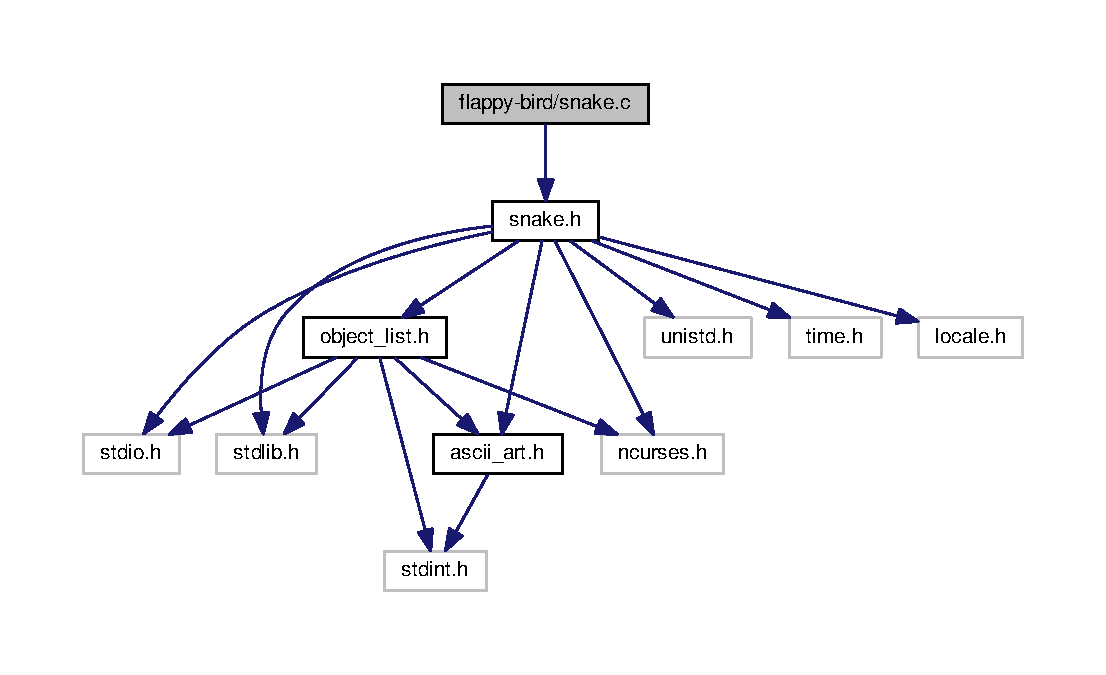
\includegraphics[width=350pt]{snake_8c__incl}
\end{center}
\end{figure}
\subsection*{Functions}
\begin{DoxyCompactItemize}
\item 
\hyperlink{structobject__list__t}{object\+\_\+list\+\_\+t} $\ast$ \hyperlink{snake_8c_a762b57e20d9c7f2d75f7c67f72e839cf}{init\+\_\+game} (void)
\begin{DoxyCompactList}\small\item\em Initailises a game state for a snake game. \end{DoxyCompactList}\item 
void \hyperlink{snake_8c_a3564187b6b7de79c8346e9345f80ad69}{move\+\_\+snake} (\hyperlink{structobject__list__t}{object\+\_\+list\+\_\+t} $\ast$list, \hyperlink{structvector__t}{vector\+\_\+t} dir)
\begin{DoxyCompactList}\small\item\em Moves the snake. \end{DoxyCompactList}\item 
void \hyperlink{snake_8c_a995012df8b3820f107bf72f57c32a523}{hit\+\_\+apple} (\hyperlink{structobject__list__t}{object\+\_\+list\+\_\+t} $\ast$list)
\begin{DoxyCompactList}\small\item\em Checks if apple is hit, creates new apple if it is. \end{DoxyCompactList}\item 
void \hyperlink{snake_8c_a7221128788d757397cdb69aed835df5c}{render\+\_\+game} (\hyperlink{structobject__list__t}{object\+\_\+list\+\_\+t} $\ast$list, \hyperlink{structvector__t}{vector\+\_\+t} dir)
\begin{DoxyCompactList}\small\item\em Renders the game, and updates the game state. \end{DoxyCompactList}\item 
int \hyperlink{snake_8c_a0b885d532e21322ee502295347a1f014}{snake\+\_\+hit} (\hyperlink{structobject__list__t}{object\+\_\+list\+\_\+t} $\ast$list)
\begin{DoxyCompactList}\small\item\em Checks if the snake has hit itself. \end{DoxyCompactList}\end{DoxyCompactItemize}


\subsection{Detailed Description}
Functions for initialising and rendering a snake game. 



\subsection{Function Documentation}
\index{snake.\+c@{snake.\+c}!hit\+\_\+apple@{hit\+\_\+apple}}
\index{hit\+\_\+apple@{hit\+\_\+apple}!snake.\+c@{snake.\+c}}
\subsubsection[{\texorpdfstring{hit\+\_\+apple(object\+\_\+list\+\_\+t $\ast$list)}{hit_apple(object_list_t *list)}}]{\setlength{\rightskip}{0pt plus 5cm}void hit\+\_\+apple (
\begin{DoxyParamCaption}
\item[{{\bf object\+\_\+list\+\_\+t} $\ast$}]{list}
\end{DoxyParamCaption}
)}\hypertarget{snake_8c_a995012df8b3820f107bf72f57c32a523}{}\label{snake_8c_a995012df8b3820f107bf72f57c32a523}


Checks if apple is hit, creates new apple if it is. 

It also creates lengthens the snake if an apple is hit. 
\begin{DoxyParams}{Parameters}
{\em list} & The object list. \\
\hline
\end{DoxyParams}
\index{snake.\+c@{snake.\+c}!init\+\_\+game@{init\+\_\+game}}
\index{init\+\_\+game@{init\+\_\+game}!snake.\+c@{snake.\+c}}
\subsubsection[{\texorpdfstring{init\+\_\+game(void)}{init_game(void)}}]{\setlength{\rightskip}{0pt plus 5cm}{\bf object\+\_\+list\+\_\+t}$\ast$ init\+\_\+game (
\begin{DoxyParamCaption}
\item[{void}]{}
\end{DoxyParamCaption}
)}\hypertarget{snake_8c_a762b57e20d9c7f2d75f7c67f72e839cf}{}\label{snake_8c_a762b57e20d9c7f2d75f7c67f72e839cf}


Initailises a game state for a snake game. 

Initailises a game state for a flappy bird game.

\begin{DoxyReturn}{Returns}
An object list representing the initial game state. 
\end{DoxyReturn}
\index{snake.\+c@{snake.\+c}!move\+\_\+snake@{move\+\_\+snake}}
\index{move\+\_\+snake@{move\+\_\+snake}!snake.\+c@{snake.\+c}}
\subsubsection[{\texorpdfstring{move\+\_\+snake(object\+\_\+list\+\_\+t $\ast$list, vector\+\_\+t dir)}{move_snake(object_list_t *list, vector_t dir)}}]{\setlength{\rightskip}{0pt plus 5cm}void move\+\_\+snake (
\begin{DoxyParamCaption}
\item[{{\bf object\+\_\+list\+\_\+t} $\ast$}]{list, }
\item[{{\bf vector\+\_\+t}}]{dir}
\end{DoxyParamCaption}
)}\hypertarget{snake_8c_a3564187b6b7de79c8346e9345f80ad69}{}\label{snake_8c_a3564187b6b7de79c8346e9345f80ad69}


Moves the snake. 


\begin{DoxyParams}{Parameters}
{\em list} & The object list. \\
\hline
{\em dir} & Direction for the snake head to go. \\
\hline
\end{DoxyParams}
\index{snake.\+c@{snake.\+c}!render\+\_\+game@{render\+\_\+game}}
\index{render\+\_\+game@{render\+\_\+game}!snake.\+c@{snake.\+c}}
\subsubsection[{\texorpdfstring{render\+\_\+game(object\+\_\+list\+\_\+t $\ast$list, vector\+\_\+t dir)}{render_game(object_list_t *list, vector_t dir)}}]{\setlength{\rightskip}{0pt plus 5cm}void render\+\_\+game (
\begin{DoxyParamCaption}
\item[{{\bf object\+\_\+list\+\_\+t} $\ast$}]{list, }
\item[{{\bf vector\+\_\+t}}]{dir}
\end{DoxyParamCaption}
)}\hypertarget{snake_8c_a7221128788d757397cdb69aed835df5c}{}\label{snake_8c_a7221128788d757397cdb69aed835df5c}


Renders the game, and updates the game state. 


\begin{DoxyParams}{Parameters}
{\em list} & The object list. \\
\hline
{\em dir} & Direction for the snake head to go. \\
\hline
\end{DoxyParams}
\index{snake.\+c@{snake.\+c}!snake\+\_\+hit@{snake\+\_\+hit}}
\index{snake\+\_\+hit@{snake\+\_\+hit}!snake.\+c@{snake.\+c}}
\subsubsection[{\texorpdfstring{snake\+\_\+hit(object\+\_\+list\+\_\+t $\ast$list)}{snake_hit(object_list_t *list)}}]{\setlength{\rightskip}{0pt plus 5cm}int snake\+\_\+hit (
\begin{DoxyParamCaption}
\item[{{\bf object\+\_\+list\+\_\+t} $\ast$}]{list}
\end{DoxyParamCaption}
)}\hypertarget{snake_8c_a0b885d532e21322ee502295347a1f014}{}\label{snake_8c_a0b885d532e21322ee502295347a1f014}


Checks if the snake has hit itself. 


\begin{DoxyParams}{Parameters}
{\em list} & The object list. \\
\hline
\end{DoxyParams}

\hypertarget{snake_8h}{}\section{flappy-\/bird/snake.h File Reference}
\label{snake_8h}\index{flappy-\/bird/snake.\+h@{flappy-\/bird/snake.\+h}}


Header file for \hyperlink{snake_8c}{snake.\+c}.  


{\ttfamily \#include $<$stdio.\+h$>$}\\*
{\ttfamily \#include $<$stdlib.\+h$>$}\\*
{\ttfamily \#include $<$unistd.\+h$>$}\\*
{\ttfamily \#include $<$time.\+h$>$}\\*
{\ttfamily \#include $<$ncurses.\+h$>$}\\*
{\ttfamily \#include \char`\"{}ascii\+\_\+art.\+h\char`\"{}}\\*
{\ttfamily \#include \char`\"{}object\+\_\+list.\+h\char`\"{}}\\*
{\ttfamily \#include $<$locale.\+h$>$}\\*
Include dependency graph for snake.\+h\+:\nopagebreak
\begin{figure}[H]
\begin{center}
\leavevmode
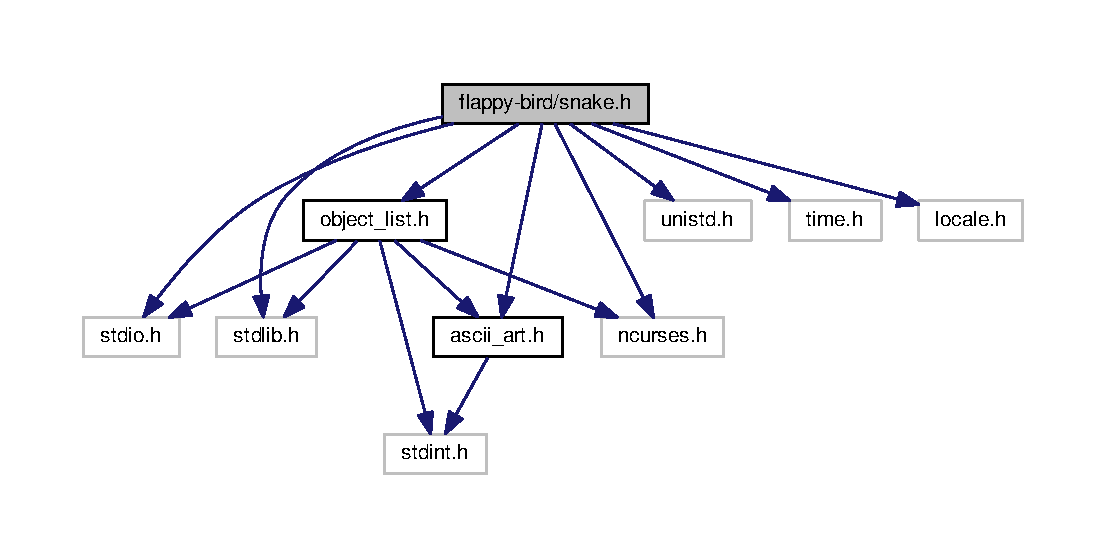
\includegraphics[width=350pt]{snake_8h__incl}
\end{center}
\end{figure}
This graph shows which files directly or indirectly include this file\+:\nopagebreak
\begin{figure}[H]
\begin{center}
\leavevmode
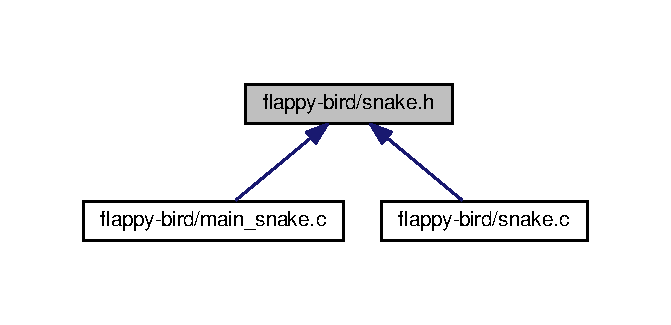
\includegraphics[width=322pt]{snake_8h__dep__incl}
\end{center}
\end{figure}
\subsection*{Macros}
\begin{DoxyCompactItemize}
\item 
\#define \hyperlink{snake_8h_a241aeeb764887ae5e3de58b98f04b16d}{W\+I\+D\+TH}~50
\item 
\#define \hyperlink{snake_8h_aed89bd71aee8be823e8a20ec4e093c1e}{H\+E\+I\+G\+HT}~50
\end{DoxyCompactItemize}
\subsection*{Functions}
\begin{DoxyCompactItemize}
\item 
int \hyperlink{snake_8h_a0b885d532e21322ee502295347a1f014}{snake\+\_\+hit} (\hyperlink{structobject__list__t}{object\+\_\+list\+\_\+t} $\ast$list)
\begin{DoxyCompactList}\small\item\em Checks if the snake has hit itself. \end{DoxyCompactList}\item 
\hyperlink{structobject__list__t}{object\+\_\+list\+\_\+t} $\ast$ \hyperlink{snake_8h_a762b57e20d9c7f2d75f7c67f72e839cf}{init\+\_\+game} (void)
\begin{DoxyCompactList}\small\item\em Initailises a game state for a flappy bird game. \end{DoxyCompactList}\item 
void \hyperlink{snake_8h_a3564187b6b7de79c8346e9345f80ad69}{move\+\_\+snake} (\hyperlink{structobject__list__t}{object\+\_\+list\+\_\+t} $\ast$list, \hyperlink{structvector__t}{vector\+\_\+t} dir)
\begin{DoxyCompactList}\small\item\em Moves the snake. \end{DoxyCompactList}\item 
void \hyperlink{snake_8h_a7221128788d757397cdb69aed835df5c}{render\+\_\+game} (\hyperlink{structobject__list__t}{object\+\_\+list\+\_\+t} $\ast$list, \hyperlink{structvector__t}{vector\+\_\+t} dir)
\begin{DoxyCompactList}\small\item\em Renders the game, and updates the game state. \end{DoxyCompactList}\item 
void \hyperlink{snake_8h_a995012df8b3820f107bf72f57c32a523}{hit\+\_\+apple} (\hyperlink{structobject__list__t}{object\+\_\+list\+\_\+t} $\ast$list)
\begin{DoxyCompactList}\small\item\em Checks if apple is hit, creates new apple if it is. \end{DoxyCompactList}\end{DoxyCompactItemize}


\subsection{Detailed Description}
Header file for \hyperlink{snake_8c}{snake.\+c}. 



\subsection{Macro Definition Documentation}
\index{snake.\+h@{snake.\+h}!H\+E\+I\+G\+HT@{H\+E\+I\+G\+HT}}
\index{H\+E\+I\+G\+HT@{H\+E\+I\+G\+HT}!snake.\+h@{snake.\+h}}
\subsubsection[{\texorpdfstring{H\+E\+I\+G\+HT}{HEIGHT}}]{\setlength{\rightskip}{0pt plus 5cm}\#define H\+E\+I\+G\+HT~50}\hypertarget{snake_8h_aed89bd71aee8be823e8a20ec4e093c1e}{}\label{snake_8h_aed89bd71aee8be823e8a20ec4e093c1e}
Height of the game. \index{snake.\+h@{snake.\+h}!W\+I\+D\+TH@{W\+I\+D\+TH}}
\index{W\+I\+D\+TH@{W\+I\+D\+TH}!snake.\+h@{snake.\+h}}
\subsubsection[{\texorpdfstring{W\+I\+D\+TH}{WIDTH}}]{\setlength{\rightskip}{0pt plus 5cm}\#define W\+I\+D\+TH~50}\hypertarget{snake_8h_a241aeeb764887ae5e3de58b98f04b16d}{}\label{snake_8h_a241aeeb764887ae5e3de58b98f04b16d}
Width of the game. 

\subsection{Function Documentation}
\index{snake.\+h@{snake.\+h}!hit\+\_\+apple@{hit\+\_\+apple}}
\index{hit\+\_\+apple@{hit\+\_\+apple}!snake.\+h@{snake.\+h}}
\subsubsection[{\texorpdfstring{hit\+\_\+apple(object\+\_\+list\+\_\+t $\ast$list)}{hit_apple(object_list_t *list)}}]{\setlength{\rightskip}{0pt plus 5cm}void hit\+\_\+apple (
\begin{DoxyParamCaption}
\item[{{\bf object\+\_\+list\+\_\+t} $\ast$}]{list}
\end{DoxyParamCaption}
)}\hypertarget{snake_8h_a995012df8b3820f107bf72f57c32a523}{}\label{snake_8h_a995012df8b3820f107bf72f57c32a523}


Checks if apple is hit, creates new apple if it is. 

It also creates lengthens the snake if an apple is hit. 
\begin{DoxyParams}{Parameters}
{\em list} & The object list. \\
\hline
\end{DoxyParams}
\index{snake.\+h@{snake.\+h}!init\+\_\+game@{init\+\_\+game}}
\index{init\+\_\+game@{init\+\_\+game}!snake.\+h@{snake.\+h}}
\subsubsection[{\texorpdfstring{init\+\_\+game(void)}{init_game(void)}}]{\setlength{\rightskip}{0pt plus 5cm}{\bf object\+\_\+list\+\_\+t}$\ast$ init\+\_\+game (
\begin{DoxyParamCaption}
\item[{void}]{}
\end{DoxyParamCaption}
)}\hypertarget{snake_8h_a762b57e20d9c7f2d75f7c67f72e839cf}{}\label{snake_8h_a762b57e20d9c7f2d75f7c67f72e839cf}


Initailises a game state for a flappy bird game. 

\begin{DoxyReturn}{Returns}
An object list representing the initial game state.
\end{DoxyReturn}
Initailises a game state for a flappy bird game.

\begin{DoxyReturn}{Returns}
An object list representing the initial game state.

An object list representing the initial game state.
\end{DoxyReturn}
Initailises a game state for a flappy bird game.

\begin{DoxyReturn}{Returns}
An object list representing the initial game state. 
\end{DoxyReturn}
\index{snake.\+h@{snake.\+h}!move\+\_\+snake@{move\+\_\+snake}}
\index{move\+\_\+snake@{move\+\_\+snake}!snake.\+h@{snake.\+h}}
\subsubsection[{\texorpdfstring{move\+\_\+snake(object\+\_\+list\+\_\+t $\ast$list, vector\+\_\+t dir)}{move_snake(object_list_t *list, vector_t dir)}}]{\setlength{\rightskip}{0pt plus 5cm}void move\+\_\+snake (
\begin{DoxyParamCaption}
\item[{{\bf object\+\_\+list\+\_\+t} $\ast$}]{list, }
\item[{{\bf vector\+\_\+t}}]{dir}
\end{DoxyParamCaption}
)}\hypertarget{snake_8h_a3564187b6b7de79c8346e9345f80ad69}{}\label{snake_8h_a3564187b6b7de79c8346e9345f80ad69}


Moves the snake. 


\begin{DoxyParams}{Parameters}
{\em list} & The object list. \\
\hline
{\em dir} & Direction for the snake head to go. \\
\hline
\end{DoxyParams}
\index{snake.\+h@{snake.\+h}!render\+\_\+game@{render\+\_\+game}}
\index{render\+\_\+game@{render\+\_\+game}!snake.\+h@{snake.\+h}}
\subsubsection[{\texorpdfstring{render\+\_\+game(object\+\_\+list\+\_\+t $\ast$list, vector\+\_\+t dir)}{render_game(object_list_t *list, vector_t dir)}}]{\setlength{\rightskip}{0pt plus 5cm}void render\+\_\+game (
\begin{DoxyParamCaption}
\item[{{\bf object\+\_\+list\+\_\+t} $\ast$}]{list, }
\item[{{\bf vector\+\_\+t}}]{dir}
\end{DoxyParamCaption}
)}\hypertarget{snake_8h_a7221128788d757397cdb69aed835df5c}{}\label{snake_8h_a7221128788d757397cdb69aed835df5c}


Renders the game, and updates the game state. 


\begin{DoxyParams}{Parameters}
{\em list} & The object list. \\
\hline
{\em dir} & Direction for the snake head to go. \\
\hline
\end{DoxyParams}
\index{snake.\+h@{snake.\+h}!snake\+\_\+hit@{snake\+\_\+hit}}
\index{snake\+\_\+hit@{snake\+\_\+hit}!snake.\+h@{snake.\+h}}
\subsubsection[{\texorpdfstring{snake\+\_\+hit(object\+\_\+list\+\_\+t $\ast$list)}{snake_hit(object_list_t *list)}}]{\setlength{\rightskip}{0pt plus 5cm}int snake\+\_\+hit (
\begin{DoxyParamCaption}
\item[{{\bf object\+\_\+list\+\_\+t} $\ast$}]{list}
\end{DoxyParamCaption}
)}\hypertarget{snake_8h_a0b885d532e21322ee502295347a1f014}{}\label{snake_8h_a0b885d532e21322ee502295347a1f014}


Checks if the snake has hit itself. 


\begin{DoxyParams}{Parameters}
{\em list} & The object list. \\
\hline
\end{DoxyParams}

\hypertarget{main_8cpp}{}\section{main.\+cpp File Reference}
\label{main_8cpp}\index{main.\+cpp@{main.\+cpp}}


Main file for motion-\/controlled games.  


{\ttfamily \#include $<$math.\+h$>$}\\*
{\ttfamily \#include $<$unistd.\+h$>$}\\*
{\ttfamily \#include \char`\"{}cv.\+h\char`\"{}}\\*
{\ttfamily \#include \char`\"{}highgui.\+h\char`\"{}}\\*
{\ttfamily \#include \char`\"{}uchar\+\_\+array.\+c\char`\"{}}\\*
{\ttfamily \#include \char`\"{}calibration.\+c\char`\"{}}\\*
{\ttfamily \#include \char`\"{}threshold.\+c\char`\"{}}\\*
{\ttfamily \#include \char`\"{}detection.\+c\char`\"{}}\\*
{\ttfamily \#include \char`\"{}flappy\+\_\+bird.\+c\char`\"{}}\\*
Include dependency graph for main.\+cpp\+:\nopagebreak
\begin{figure}[H]
\begin{center}
\leavevmode
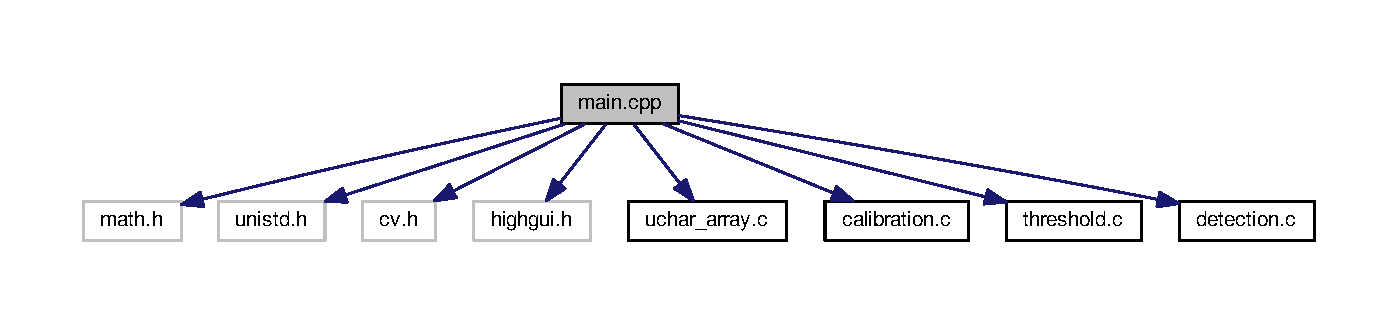
\includegraphics[width=350pt]{main_8cpp__incl}
\end{center}
\end{figure}
\subsection*{Functions}
\begin{DoxyCompactItemize}
\item 
void {\bfseries generate\+\_\+movement\+\_\+frame} (Ipl\+Image $\ast$debug\+\_\+frame, const Ipl\+Image $\ast$prev\+\_\+frame, const Ipl\+Image $\ast$frame)\hypertarget{main_8cpp_a2018a460a34a69628f62e71b6ad3677a}{}\label{main_8cpp_a2018a460a34a69628f62e71b6ad3677a}

\item 
int {\bfseries main} (int argc, char $\ast$$\ast$argv)\hypertarget{main_8cpp_a3c04138a5bfe5d72780bb7e82a18e627}{}\label{main_8cpp_a3c04138a5bfe5d72780bb7e82a18e627}

\end{DoxyCompactItemize}


\subsection{Detailed Description}
Main file for motion-\/controlled games. 


\hypertarget{threshold_8c}{}\section{threshold.\+c File Reference}
\label{threshold_8c}\index{threshold.\+c@{threshold.\+c}}


Functions to determine skin-\/coloured pixel within a frame.  


This graph shows which files directly or indirectly include this file\+:\nopagebreak
\begin{figure}[H]
\begin{center}
\leavevmode
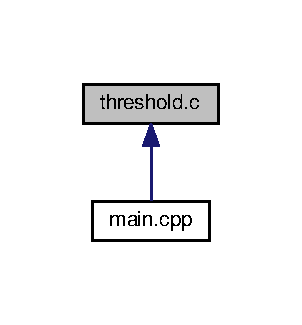
\includegraphics[width=145pt]{threshold_8c__dep__incl}
\end{center}
\end{figure}
\subsection*{Functions}
\begin{DoxyCompactItemize}
\item 
bool \hyperlink{threshold_8c_a79eb57ff62bb45178ac15c08b15ed27e}{in\+\_\+range} (unsigned char value, unsigned char min, unsigned char \hyperlink{uchar__array_8c_aa8aa6047ffa6af174d25a687952014d6}{max}, unsigned char range)
\begin{DoxyCompactList}\small\item\em Checks whether a given value is in a given range. Note that the minimum and maximum values can sometimes be swapped due to the fact that H\+SV is circular. \end{DoxyCompactList}\item 
Ipl\+Image $\ast$ \hyperlink{threshold_8c_ad5e2bed0c06e751ec19877291c7043cb}{get\+\_\+arm} (Ipl\+Image $\ast$frame, \hyperlink{structcalibration__t}{calibration\+\_\+t} $\ast$c)
\begin{DoxyCompactList}\small\item\em Gets a black and white frame of where the skin is. Given a frame and a calibration struct, it marks each pixel white where skin is present. \end{DoxyCompactList}\item 
double \hyperlink{threshold_8c_afd858b40efaa1559c3325b0cb5f5cd1c}{dist} (int x1, int x2, int y1, int y2, int z1, int z2)
\begin{DoxyCompactList}\small\item\em Finds distance between 2 points in 3D space. \end{DoxyCompactList}\end{DoxyCompactItemize}


\subsection{Detailed Description}
Functions to determine skin-\/coloured pixel within a frame. 



\subsection{Function Documentation}
\index{threshold.\+c@{threshold.\+c}!dist@{dist}}
\index{dist@{dist}!threshold.\+c@{threshold.\+c}}
\subsubsection[{\texorpdfstring{dist(int x1, int x2, int y1, int y2, int z1, int z2)}{dist(int x1, int x2, int y1, int y2, int z1, int z2)}}]{\setlength{\rightskip}{0pt plus 5cm}double dist (
\begin{DoxyParamCaption}
\item[{int}]{x1, }
\item[{int}]{x2, }
\item[{int}]{y1, }
\item[{int}]{y2, }
\item[{int}]{z1, }
\item[{int}]{z2}
\end{DoxyParamCaption}
)}\hypertarget{threshold_8c_afd858b40efaa1559c3325b0cb5f5cd1c}{}\label{threshold_8c_afd858b40efaa1559c3325b0cb5f5cd1c}


Finds distance between 2 points in 3D space. 


\begin{DoxyParams}{Parameters}
{\em x1} & The x coordinate of the first point. \\
\hline
{\em x2} & The x coordinate of the second point. \\
\hline
{\em y1} & The y coordinate of the first point. \\
\hline
{\em y2} & The y coordinate of the second point. \\
\hline
{\em z1} & The z coordinate of the first point. \\
\hline
{\em z2} & The z coordinate of the second point. \\
\hline
\end{DoxyParams}
\begin{DoxyReturn}{Returns}
The distance between the 2 point. 
\end{DoxyReturn}
\index{threshold.\+c@{threshold.\+c}!get\+\_\+arm@{get\+\_\+arm}}
\index{get\+\_\+arm@{get\+\_\+arm}!threshold.\+c@{threshold.\+c}}
\subsubsection[{\texorpdfstring{get\+\_\+arm(\+Ipl\+Image $\ast$frame, calibration\+\_\+t $\ast$c)}{get_arm(IplImage *frame, calibration_t *c)}}]{\setlength{\rightskip}{0pt plus 5cm}Ipl\+Image$\ast$ get\+\_\+arm (
\begin{DoxyParamCaption}
\item[{Ipl\+Image $\ast$}]{frame, }
\item[{{\bf calibration\+\_\+t} $\ast$}]{c}
\end{DoxyParamCaption}
)}\hypertarget{threshold_8c_ad5e2bed0c06e751ec19877291c7043cb}{}\label{threshold_8c_ad5e2bed0c06e751ec19877291c7043cb}


Gets a black and white frame of where the skin is. Given a frame and a calibration struct, it marks each pixel white where skin is present. 


\begin{DoxyParams}{Parameters}
{\em frame} & The Ipl\+Image frame. \\
\hline
{\em c} & The calibration which contains the skin colour. \\
\hline
\end{DoxyParams}
\begin{DoxyReturn}{Returns}
A black and white Ipl\+Image frame indicating where skin is. 
\end{DoxyReturn}
\index{threshold.\+c@{threshold.\+c}!in\+\_\+range@{in\+\_\+range}}
\index{in\+\_\+range@{in\+\_\+range}!threshold.\+c@{threshold.\+c}}
\subsubsection[{\texorpdfstring{in\+\_\+range(unsigned char value, unsigned char min, unsigned char max, unsigned char range)}{in_range(unsigned char value, unsigned char min, unsigned char max, unsigned char range)}}]{\setlength{\rightskip}{0pt plus 5cm}bool in\+\_\+range (
\begin{DoxyParamCaption}
\item[{unsigned char}]{value, }
\item[{unsigned char}]{min, }
\item[{unsigned char}]{max, }
\item[{unsigned char}]{range}
\end{DoxyParamCaption}
)}\hypertarget{threshold_8c_a79eb57ff62bb45178ac15c08b15ed27e}{}\label{threshold_8c_a79eb57ff62bb45178ac15c08b15ed27e}


Checks whether a given value is in a given range. Note that the minimum and maximum values can sometimes be swapped due to the fact that H\+SV is circular. 


\begin{DoxyParams}{Parameters}
{\em value} & The value to check whether it is in range. \\
\hline
{\em min} & Normally the minimum value to accept. \\
\hline
{\em max} & Normally the maximum value to accept. \\
\hline
{\em range} & The maximum value that is allowed. \\
\hline
\end{DoxyParams}
\begin{DoxyReturn}{Returns}
True iff the value is in the specified range. 
\end{DoxyReturn}

\hypertarget{uchar__array_8c}{}\section{uchar\+\_\+array.\+c File Reference}
\label{uchar__array_8c}\index{uchar\+\_\+array.\+c@{uchar\+\_\+array.\+c}}


Definition of and functions for unsigned character array.  


This graph shows which files directly or indirectly include this file\+:\nopagebreak
\begin{figure}[H]
\begin{center}
\leavevmode
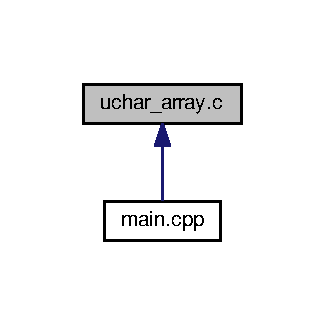
\includegraphics[width=156pt]{uchar__array_8c__dep__incl}
\end{center}
\end{figure}
\subsection*{Data Structures}
\begin{DoxyCompactItemize}
\item 
struct \hyperlink{structuchar__array__t}{uchar\+\_\+array\+\_\+t}
\begin{DoxyCompactList}\small\item\em A struct to hold a unsigned char array. Also holds the size, and the standard deviation. \end{DoxyCompactList}\end{DoxyCompactItemize}
\subsection*{Functions}
\begin{DoxyCompactItemize}
\item 
unsigned char \hyperlink{uchar__array_8c_aa8aa6047ffa6af174d25a687952014d6}{max} (\hyperlink{structuchar__array__t}{uchar\+\_\+array\+\_\+t} $\ast$data)
\begin{DoxyCompactList}\small\item\em Finds the maximum value inside a given unsigned char array. Note that if the array is empty then the maximum value is zero. \end{DoxyCompactList}\item 
double \hyperlink{uchar__array_8c_a50552ea1e39782dc965895b0f0b3e8e6}{avg} (\hyperlink{structuchar__array__t}{uchar\+\_\+array\+\_\+t} $\ast$data)
\begin{DoxyCompactList}\small\item\em Finds the average value of a given unsigned char array. \end{DoxyCompactList}\item 
void \hyperlink{uchar__array_8c_a21e9524031b40a15fca0fa9a51493576}{standard\+\_\+dev} (\hyperlink{structuchar__array__t}{uchar\+\_\+array\+\_\+t} $\ast$data)
\begin{DoxyCompactList}\small\item\em Sets the standard deviation of a given \hyperlink{structuchar__array__t}{uchar\+\_\+array\+\_\+t} struct. \end{DoxyCompactList}\item 
unsigned char \hyperlink{uchar__array_8c_ac65bb7dcd66d8fedef18465aae7192b6}{lower} (\hyperlink{structuchar__array__t}{uchar\+\_\+array\+\_\+t} $\ast$data, double dev)
\begin{DoxyCompactList}\small\item\em Finds the lower quartile of a given unsigned char array. \end{DoxyCompactList}\item 
unsigned char \hyperlink{uchar__array_8c_a7d2bd11f8ff2cdddcc17eb20f5ca0f22}{upper} (\hyperlink{structuchar__array__t}{uchar\+\_\+array\+\_\+t} $\ast$data, double dev)
\begin{DoxyCompactList}\small\item\em Finds the upper quartile of a given unsigned char array. \end{DoxyCompactList}\item 
\hyperlink{structuchar__array__t}{uchar\+\_\+array\+\_\+t} $\ast$ \hyperlink{uchar__array_8c_a42f3a0201ba1b1fcea1554356da70aaa}{init\+\_\+arr} (int size)
\begin{DoxyCompactList}\small\item\em Initialises a \hyperlink{structuchar__array__t}{uchar\+\_\+array\+\_\+t} struct. \end{DoxyCompactList}\end{DoxyCompactItemize}


\subsection{Detailed Description}
Definition of and functions for unsigned character array. 



\subsection{Function Documentation}
\index{uchar\+\_\+array.\+c@{uchar\+\_\+array.\+c}!avg@{avg}}
\index{avg@{avg}!uchar\+\_\+array.\+c@{uchar\+\_\+array.\+c}}
\subsubsection[{\texorpdfstring{avg(uchar\+\_\+array\+\_\+t $\ast$data)}{avg(uchar_array_t *data)}}]{\setlength{\rightskip}{0pt plus 5cm}double avg (
\begin{DoxyParamCaption}
\item[{{\bf uchar\+\_\+array\+\_\+t} $\ast$}]{data}
\end{DoxyParamCaption}
)}\hypertarget{uchar__array_8c_a50552ea1e39782dc965895b0f0b3e8e6}{}\label{uchar__array_8c_a50552ea1e39782dc965895b0f0b3e8e6}


Finds the average value of a given unsigned char array. 


\begin{DoxyParams}{Parameters}
{\em data} & The unsigned char array. \\
\hline
\end{DoxyParams}
\begin{DoxyReturn}{Returns}
The average value. 
\end{DoxyReturn}
\index{uchar\+\_\+array.\+c@{uchar\+\_\+array.\+c}!init\+\_\+arr@{init\+\_\+arr}}
\index{init\+\_\+arr@{init\+\_\+arr}!uchar\+\_\+array.\+c@{uchar\+\_\+array.\+c}}
\subsubsection[{\texorpdfstring{init\+\_\+arr(int size)}{init_arr(int size)}}]{\setlength{\rightskip}{0pt plus 5cm}{\bf uchar\+\_\+array\+\_\+t}$\ast$ init\+\_\+arr (
\begin{DoxyParamCaption}
\item[{int}]{size}
\end{DoxyParamCaption}
)}\hypertarget{uchar__array_8c_a42f3a0201ba1b1fcea1554356da70aaa}{}\label{uchar__array_8c_a42f3a0201ba1b1fcea1554356da70aaa}


Initialises a \hyperlink{structuchar__array__t}{uchar\+\_\+array\+\_\+t} struct. 


\begin{DoxyParams}{Parameters}
{\em size} & The number of elements in the array. \\
\hline
\end{DoxyParams}
\begin{DoxyReturn}{Returns}
The pointer to the initialised struct. 
\end{DoxyReturn}
\index{uchar\+\_\+array.\+c@{uchar\+\_\+array.\+c}!lower@{lower}}
\index{lower@{lower}!uchar\+\_\+array.\+c@{uchar\+\_\+array.\+c}}
\subsubsection[{\texorpdfstring{lower(uchar\+\_\+array\+\_\+t $\ast$data, double dev)}{lower(uchar_array_t *data, double dev)}}]{\setlength{\rightskip}{0pt plus 5cm}unsigned char lower (
\begin{DoxyParamCaption}
\item[{{\bf uchar\+\_\+array\+\_\+t} $\ast$}]{data, }
\item[{double}]{dev}
\end{DoxyParamCaption}
)}\hypertarget{uchar__array_8c_ac65bb7dcd66d8fedef18465aae7192b6}{}\label{uchar__array_8c_ac65bb7dcd66d8fedef18465aae7192b6}


Finds the lower quartile of a given unsigned char array. 


\begin{DoxyParams}{Parameters}
{\em data} & The unsigned char array. \\
\hline
{\em dev} & The deviation. \\
\hline
\end{DoxyParams}
\begin{DoxyReturn}{Returns}
The lower quartile. 
\end{DoxyReturn}
\index{uchar\+\_\+array.\+c@{uchar\+\_\+array.\+c}!max@{max}}
\index{max@{max}!uchar\+\_\+array.\+c@{uchar\+\_\+array.\+c}}
\subsubsection[{\texorpdfstring{max(uchar\+\_\+array\+\_\+t $\ast$data)}{max(uchar_array_t *data)}}]{\setlength{\rightskip}{0pt plus 5cm}unsigned char max (
\begin{DoxyParamCaption}
\item[{{\bf uchar\+\_\+array\+\_\+t} $\ast$}]{data}
\end{DoxyParamCaption}
)}\hypertarget{uchar__array_8c_aa8aa6047ffa6af174d25a687952014d6}{}\label{uchar__array_8c_aa8aa6047ffa6af174d25a687952014d6}


Finds the maximum value inside a given unsigned char array. Note that if the array is empty then the maximum value is zero. 


\begin{DoxyParams}{Parameters}
{\em data} & The unsigned char array. \\
\hline
\end{DoxyParams}
\begin{DoxyReturn}{Returns}
The maximum value. 
\end{DoxyReturn}
\index{uchar\+\_\+array.\+c@{uchar\+\_\+array.\+c}!standard\+\_\+dev@{standard\+\_\+dev}}
\index{standard\+\_\+dev@{standard\+\_\+dev}!uchar\+\_\+array.\+c@{uchar\+\_\+array.\+c}}
\subsubsection[{\texorpdfstring{standard\+\_\+dev(uchar\+\_\+array\+\_\+t $\ast$data)}{standard_dev(uchar_array_t *data)}}]{\setlength{\rightskip}{0pt plus 5cm}void standard\+\_\+dev (
\begin{DoxyParamCaption}
\item[{{\bf uchar\+\_\+array\+\_\+t} $\ast$}]{data}
\end{DoxyParamCaption}
)}\hypertarget{uchar__array_8c_a21e9524031b40a15fca0fa9a51493576}{}\label{uchar__array_8c_a21e9524031b40a15fca0fa9a51493576}


Sets the standard deviation of a given \hyperlink{structuchar__array__t}{uchar\+\_\+array\+\_\+t} struct. 


\begin{DoxyParams}{Parameters}
{\em data} & The \hyperlink{structuchar__array__t}{uchar\+\_\+array\+\_\+t} struct. \\
\hline
\end{DoxyParams}
\index{uchar\+\_\+array.\+c@{uchar\+\_\+array.\+c}!upper@{upper}}
\index{upper@{upper}!uchar\+\_\+array.\+c@{uchar\+\_\+array.\+c}}
\subsubsection[{\texorpdfstring{upper(uchar\+\_\+array\+\_\+t $\ast$data, double dev)}{upper(uchar_array_t *data, double dev)}}]{\setlength{\rightskip}{0pt plus 5cm}unsigned char upper (
\begin{DoxyParamCaption}
\item[{{\bf uchar\+\_\+array\+\_\+t} $\ast$}]{data, }
\item[{double}]{dev}
\end{DoxyParamCaption}
)}\hypertarget{uchar__array_8c_a7d2bd11f8ff2cdddcc17eb20f5ca0f22}{}\label{uchar__array_8c_a7d2bd11f8ff2cdddcc17eb20f5ca0f22}


Finds the upper quartile of a given unsigned char array. 


\begin{DoxyParams}{Parameters}
{\em data} & The unsigned char array. \\
\hline
{\em dev} & The deviation. \\
\hline
\end{DoxyParams}
\begin{DoxyReturn}{Returns}
The upper quartile. 
\end{DoxyReturn}

%--- End generated contents ---

% Index
\backmatter
\newpage
\phantomsection
\clearemptydoublepage
\addcontentsline{toc}{chapter}{Index}
\printindex

\end{document}
